%%%%%%%%%%%%%%%%%%%%%%%%%%%%%%%%%%%%%%%%%%%%%%%%%%%%%%%%%%%%%%%%%%%%%%
% Template for a UBC-compliant dissertation
% At the minimum, you will need to change the information found
% after the "Document meta-data"
%
%!TEX TS-program = pdflatex
%!TEX encoding = UTF-8 Unicode

%% The ubcdiss class provides several options:
%%   gpscopy (aka fogscopy)
%%       set parameters to exactly how GPS specifies
%%         * single-sided
%%         * page-numbering starts from title page
%%         * the lists of figures and tables have each entry prefixed
%%           with 'Figure' or 'Table'
%%       This can be tested by `\ifgpscopy ... \else ... \fi'
%%   10pt, 11pt, 12pt
%%       set default font size
%%   oneside, twoside
%%       whether to format for single-sided or double-sided printing
%%   balanced
%%       when double-sided, ensure page content is centred
%%       rather than slightly offset (the default)
%%   singlespacing, onehalfspacing, doublespacing
%%       set default inter-line text spacing; the ubcdiss class
%%       provides \textspacing to revert to this configured spacing
%%   draft
%%       disable more intensive processing, such as including
%%       graphics, etc.
%%

% For submission to GPS
\documentclass[gpscopy,onehalfspacing,11pt]{ubcdiss}

% For your own copies (looks nicer)
% \documentclass[balanced,twoside,11pt]{ubcdiss}

%%%%%%%%%%%%%%%%%%%%%%%%%%%%%%%%%%%%%%%%%%%%%%%%%%%%%%%%%%%%%%%%%%%%%%
%%%%%%%%%%%%%%%%%%%%%%%%%%%%%%%%%%%%%%%%%%%%%%%%%%%%%%%%%%%%%%%%%%%%%%
%%
%% FONTS:
%% 
%% The defaults below configures Times Roman for the serif font,
%% Helvetica for the sans serif font, and Courier for the
%% typewriter-style font.  Configuring fonts can be time
%% consuming; we recommend skipping to END FONTS!
%% 
%% If you're feeling brave, have lots of time, and wish to use one
%% your platform's native fonts, see the commented out bits below for
%% XeTeX/XeLaTeX.  This is not for the faint at heart. 
%% (And shouldn't you be writing? :-)
%%

%% NFSS font specification (New Font Selection Scheme)
\usepackage{times,mathptmx,courier}
\usepackage[scaled=.92]{helvet}

%% Math or theory people may want to include the handy AMS macros
%\usepackage{amssymb}
%\usepackage{amsmath}
%\usepackage{amsfonts}

%% The pifont package provides access to the elements in the dingbat font.   
%% Use \ding{##} for a particular dingbat (see p7 of psnfss2e.pdf)
%%   Useful:
%%     51,52 different forms of a checkmark
%%     54,55,56 different forms of a cross (saltyre)
%%     172-181 are 1-10 in open circle (serif)
%%     182-191 are 1-10 black circle (serif)
%%     192-201 are 1-10 in open circle (sans serif)
%%     202-211 are 1-10 in black circle (sans serif)
%% \begin{dinglist}{##}\item... or dingautolist (which auto-increments)
%% to create a bullet list with the provided character.
\usepackage{pifont}

%%%%%%%%%%%%%%%%%%%%%%%%%%%%%%%%%%%%%%%%%%%%%%%%%%%%%%%%%%%%%%%%%%%%%%
%% Configure fonts for XeTeX / XeLaTeX using the fontspec package.
%% Be sure to check out the fontspec documentation.
%\usepackage{fontspec,xltxtra,xunicode}	% required
%\defaultfontfeatures{Mapping=tex-text}	% recommended
%% Minion Pro and Myriad Pro are shipped with some versions of
%% Adobe Reader.  Adobe representatives have commented that these
%% fonts can be used outside of Adobe Reader.
%\setromanfont[Numbers=OldStyle]{Minion Pro}
%\setsansfont[Numbers=OldStyle,Scale=MatchLowercase]{Myriad Pro}
%\setmonofont[Scale=MatchLowercase]{Andale Mono}

%% Other alternatives:
%\setromanfont[Mapping=tex-text]{Adobe Caslon}
%\setsansfont[Scale=MatchLowercase]{Gill Sans}
%\setsansfont[Scale=MatchLowercase,Mapping=tex-text]{Futura}
%\setmonofont[Scale=MatchLowercase]{Andale Mono}
%\newfontfamily{\SYM}[Scale=0.9]{Zapf Dingbats}
%% END FONTS
%%%%%%%%%%%%%%%%%%%%%%%%%%%%%%%%%%%%%%%%%%%%%%%%%%%%%%%%%%%%%%%%%%%%%%
%%%%%%%%%%%%%%%%%%%%%%%%%%%%%%%%%%%%%%%%%%%%%%%%%%%%%%%%%%%%%%%%%%%%%%
%\usepackage{cite}
\usepackage{amsmath,amssymb,amsfonts}
\usepackage{algorithmic}
\usepackage{graphicx}
\usepackage{textcomp}
\usepackage{xcolor}
\usepackage{xcolor,colortbl}
\usepackage[english]{babel}
\usepackage[utf8]{inputenc}
\usepackage{ragged2e}
\usepackage{subcaption}
\usepackage{blindtext}
\usepackage{balance}
 \usepackage[utf8]{inputenc}
 \usepackage[T1]{fontenc}
\usepackage[english]{babel}
\usepackage{csquotes}


%%%%%%%%%%%%%%%%%%%%%%%%%%%%%%%%%%%%%%%%%%%%%%%%%%%%%%%%%%%%%%%%%%%%%%
%%%%%%%%%%%%%%%%%%%%%%%%%%%%%%%%%%%%%%%%%%%%%%%%%%%%%%%%%%%%%%%%%%%%%%
%%
%% Recommended packages
%%
\usepackage{checkend}	% better error messages on left-open environments
\usepackage{graphicx}	% for incorporating external images

%% booktabs: provides some special commands for typesetting tables as used
%% in excellent journals.  Ignore the examples in the Lamport book!
\usepackage{booktabs}

%% listings: useful support for including source code listings, with
%% optional special keyword formatting.  The \lstset{} causes
%% the text to be typeset in a smaller sans serif font, with
%% proportional spacing.
\usepackage{listings}
\lstset{basicstyle=\sffamily\scriptsize,showstringspaces=false,fontadjust}

%% The acronym package provides support for defining acronyms, providing
%% their expansion when first used, and building glossaries.  See the
%% example in glossary.tex and the example usage throughout the example
%% document.
%% NOTE: to use \MakeTextLowercase in the \acsfont command below,
%%   we *must* use the `nohyperlinks' option -- it causes errors with
%%   hyperref otherwise.  See Section 5.2 in the ``LaTeX 2e for Class
%%   and Package Writers Guide'' (clsguide.pdf) for details.
\usepackage[printonlyused,nohyperlinks]{acronym}
%% The ubcdiss.cls loads the `textcase' package which provides commands
%% for upper-casing and lower-casing text.  The following causes
%% the acronym package to typeset acronyms in small-caps
%% as recommended by Bringhurst.
\renewcommand{\acsfont}[1]{{\scshape \MakeTextLowercase{#1}}}

%% color: add support for expressing colour models.  Grey can be used
%% to great effect to emphasize other parts of a graphic or text.
%% For an excellent set of examples, see Tufte's "Visual Display of
%% Quantitative Information" or "Envisioning Information".
\usepackage{color}
\definecolor{greytext}{gray}{0.5}

%% comment: provides a new {comment} environment: all text inside the
%% environment is ignored.
%%   \begin{comment} ignored text ... \end{comment}
\usepackage{comment}

%% The natbib package provides more sophisticated citing commands
%% such as \citeauthor{} to provide the author names of a work,
%% \citet{} to produce an author-and-reference citation,
%% \citep{} to produce a parenthetical citation.
%% We use \citeeg{} to provide examples

\usepackage[numbers,sort&compress]{natbib}

\newcommand{\citeeg}[1]{\citep[e.g.,][]{#1}}

%% The titlesec package provides commands to vary how chapter and
%% section titles are typeset.  The following uses more compact
%% spacings above and below the title.  The titleformat that follow
%% ensure chapter/section titles are set in singlespace.
\usepackage[compact]{titlesec}
\titleformat*{\section}{\singlespacing\raggedright\bfseries\Large}
\titleformat*{\subsection}{\singlespacing\raggedright\bfseries\large}
\titleformat*{\subsubsection}{\singlespacing\raggedright\bfseries}
\titleformat*{\paragraph}{\singlespacing\raggedright\itshape}

%% The caption package provides support for varying how table and
%% figure captions are typeset.
\usepackage[format=hang,indention=-1cm,labelfont={bf},margin=1em]{caption}

%% url: for typesetting URLs and smart(er) hyphenation.
%% \url{http://...} 
\usepackage{url}
\urlstyle{sf}	% typeset urls in sans-serif


%%%%%%%%%%%%%%%%%%%%%%%%%%%%%%%%%%%%%%%%%%%%%%%%%%%%%%%%%%%%%%%%%%%%%%
%%%%%%%%%%%%%%%%%%%%%%%%%%%%%%%%%%%%%%%%%%%%%%%%%%%%%%%%%%%%%%%%%%%%%%
%%
%% Possibly useful packages: you may need to explicitly install
%% these from CTAN if they aren't part of your distribution;
%% teTeX seems to ship with a smaller base than MikTeX and MacTeX.
%%
%\usepackage{pdfpages}	% insert pages from other PDF files
%\usepackage{longtable}	% provide tables spanning multiple pages
%\usepackage{chngpage}	% support changing the page widths on demand
%\usepackage{tabularx}	% an enhanced tabular environment

%% enumitem: support pausing and resuming enumerate environments.
%\usepackage{enumitem}

%% rotating: provides two environments, sidewaystable and sidewaysfigure,
%% for typesetting tables and figures in landscape mode.  
%\usepackage{rotating}

%% subfig: provides for including subfigures within a figure,
%% and includes being able to separately reference the subfigures.
%\usepackage{subfig}

%% ragged2e: provides several new new commands \Centering, \RaggedLeft,
%% \RaggedRight and \justifying and new environments Center, FlushLeft,
%% FlushRight and justify, which set ragged text and are easily
%% configurable to allow hyphenation.
%\usepackage{ragged2e}

%% The ulem package provides a \sout{} for striking out text and
%% \xout for crossing out text.  The normalem and normalbf are
%% necessary as the package messes with the emphasis and bold fonts
%% otherwise.
%\usepackage[normalem,normalbf]{ulem}    % for \sout

%%%%%%%%%%%%%%%%%%%%%%%%%%%%%%%%%%%%%%%%%%%%%%%%%%%%%%%%%%%%%%%%%%%%%%
%% HYPERREF:
%% The hyperref package provides for embedding hyperlinks into your
%% document.  By default the table of contents, references, citations,
%% and footnotes are hyperlinked.
%%
%% Hyperref provides a very handy command for doing cross-references:
%% \autoref{}.  This is similar to \ref{} and \pageref{} except that
%% it automagically puts in the *type* of reference.  For example,
%% referencing a figure's label will put the text `Figure 3.4'.
%% And the text will be hyperlinked to the appropriate place in the
%% document.
%%
%% Generally hyperref should appear after most other packages

%% The `pagebackref' causes the references in the bibliography to have
%% back-references to the citing page; `backref' puts the citing section
%% number.  See further below for other examples of using hyperref.
%% 2009/12/09: now use `linktocpage' (Jacek Kisynski): GPS now prefers
%%   that the ToC, LoF, LoT place the hyperlink on the page number,
%%   rather than the entry text.
\ifgpscopy
  % GPS requires that weblinks should be dark blue, which looks a bit
  % odd in printed form.
  % https://www.grad.ubc.ca/current-students/dissertation-thesis-preparation/fonts-print
  \usepackage[bookmarks,bookmarksnumbered,%
     pagebackref,linktocpage,%
     colorlinks=true,%
     linkcolor=black,%
     urlcolor=blue,%
     citecolor=black%
     ]{hyperref}
\else
  %% The following puts hyperlinks in very faint grey boxes (in pdf only).
  \usepackage[bookmarks,bookmarksnumbered,%
    pagebackref,linktocpage%
    allbordercolors={0.8 0.8 0.8},%
    ]{hyperref}
\fi
%% The following change how the the back-references text is typeset in a
%% bibliography when `backref' or `pagebackref' are used
%%
%% Change \nocitations if you'd like some text shown where there
%% are no citations found (e.g., pulled in with \nocite{xxx})
\newcommand{\nocitations}{\relax}
%%\newcommand{\nocitations}{No citations}
%%
%\renewcommand*{\backref}[1]{}% necessary for backref < 1.33
\renewcommand*{\backrefsep}{,~}%
\renewcommand*{\backreftwosep}{,~}% ', and~'
\renewcommand*{\backreflastsep}{,~}% ' and~'
\renewcommand*{\backrefalt}[4]{%
\textcolor{greytext}{\ifcase #1%
\nocitations%
\or
\(\rightarrow\) page #2%
\else
\(\rightarrow\) pages #2%
\fi}}


%% The following uses most defaults, which causes hyperlinks to be
%% surrounded by colourful boxes; the colours are only visible in
%% PDFs and don't show up when printed:
%\usepackage[bookmarks,bookmarksnumbered]{hyperref}

%% The following disables the colourful boxes around hyperlinks.
%\usepackage[bookmarks,bookmarksnumbered,pdfborder={0 0 0}]{hyperref}

%% The following disables all hyperlinking, but still enabled use of
%% \autoref{}
%\usepackage[draft]{hyperref}

%% The following commands causes chapter and section references to
%% uppercase the part name.
\renewcommand{\chapterautorefname}{Chapter}
\renewcommand{\sectionautorefname}{Section}
\renewcommand{\subsectionautorefname}{Section}
\renewcommand{\subsubsectionautorefname}{Section}

%% If you have long page numbers (e.g., roman numbers in the 
%% preliminary pages for page 28 = xxviii), you might need to
%% uncomment the following and tweak the \@pnumwidth length
%% (default: 1.55em).  See the tocloft documentation at
%% http://www.ctan.org/tex-archive/macros/latex/contrib/tocloft/
% \makeatletter
% \renewcommand{\@pnumwidth}{3em}
% \makeatother

%%%%%%%%%%%%%%%%%%%%%%%%%%%%%%%%%%%%%%%%%%%%%%%%%%%%%%%%%%%%%%%%%%%%%%
%%%%%%%%%%%%%%%%%%%%%%%%%%%%%%%%%%%%%%%%%%%%%%%%%%%%%%%%%%%%%%%%%%%%%%
%%
%% Some special settings that controls how text is typeset
%%
% \raggedbottom		% pages don't have to line up nicely on the last line
% \sloppy		% be a bit more relaxed in inter-word spacing
% \clubpenalty=10000	% try harder to avoid orphans
% \widowpenalty=10000	% try harder to avoid widows
% \tolerance=1000

%% And include some of our own useful macros
\input{macros}

%%%%%%%%%%%%%%%%%%%%%%%%%%%%%%%%%%%%%%%%%%%%%%%%%%%%%%%%%%%%%%%%%%%%%%
%%%%%%%%%%%%%%%%%%%%%%%%%%%%%%%%%%%%%%%%%%%%%%%%%%%%%%%%%%%%%%%%%%%%%%
%%
%% Document meta-data: be sure to also change the \hypersetup information
%%

\title{IoT Bugs and Development Challenges}
%\subtitle{If you want a subtitle}

\author{Amir Makhshari}
\previousdegree{B. Basket Weaving, University of Illustrious Arts, 1991}
\previousdegree{M. Silly Walks, Another University, 1994}

% What is this dissertation for?
\degreetitle{Doctor of Philosophy}

\institution{The University of British Columbia}
\campus{Vancouver}

\faculty{The Faculty of Applied Science}
\department{Electrical and Computer Engineering}
\submissionmonth{July}
\submissionyear{2021}

% details of your examining committee
\examiningcommittee{Ali Mesbah}{Supervisor}
\examiningcommittee{Karthik Pattabiraman}%
    {Supervisory Committee Member}
\examiningcommittee{Nebulous Name, Department}{Supervisory Committee Member}
\examiningcommittee{Magnus Monolith, Other Department}{Additional Examiner}

% details of your supervisory committee
\supervisorycommittee{Ira Crater, Materials Engineering}%
    {Supervisory Committee Member}
\supervisorycommittee{Adeline Long, \textsc{CEO} of Aerial Machine
    Transportation, Inc.}{Supervisory Committee Member}

%% hyperref package provides support for embedding meta-data in .PDF
%% files
\hypersetup{
  pdftitle={Change this title!  (DRAFT: \today)},
  pdfauthor={Johnny Canuck},
  pdfkeywords={Your keywords here}
}

%%%%%%%%%%%%%%%%%%%%%%%%%%%%%%%%%%%%%%%%%%%%%%%%%%%%%%%%%%%%%%%%%%%%%%
%%%%%%%%%%%%%%%%%%%%%%%%%%%%%%%%%%%%%%%%%%%%%%%%%%%%%%%%%%%%%%%%%%%%%%
%% 
%% The document content
%%

%% LaTeX's \includeonly commands causes any uses of \include{} to only
%% include files that are in the list.  This is helpful to produce
%% subsets of your thesis (e.g., for committee members who want to see
%% the dissertation chapter by chapter).  It also saves time by 
%% avoiding reprocessing the entire file.
%\includeonly{intro,conclusions}
%\includeonly{discussion}

\begin{document}

%%%%%%%%%%%%%%%%%%%%%%%%%%%%%%%%%%%%%%%%%%%%%%%%%%
%% From Thesis Components: Tradtional Thesis
%% <http://www.grad.ubc.ca/current-students/dissertation-thesis-preparation/order-components>

% Preliminary Pages (numbered in lower case Roman numerals)
%    1. Title page (mandatory)
\maketitle

%    2. Committee page (mandatory): lists supervisory committee and,
%    if applicable, the examining committee
\makecommitteepage

%    3. Abstract (mandatory - maximum 350 words)
%% The following is a directive for TeXShop to indicate the main file
%%!TEX root = diss.tex

\chapter{Abstract}

IoT systems are rapidly adopted in various domains, from embedded systems to smart homes. Despite their growing adoption and popularity, there has been no thorough study to understand IoT development challenges from the practitioners' point of view. We provide the first systematic study of bugs and challenges that IoT developers face in practice, through a large-scale empirical investigation. We collected 5,565 bug reports from 91 representative IoT project repositories and categorized a random sample of 323 based on the observed failures, root causes, and the locations of the faulty components. In addition, we conducted nine interviews with IoT experts to uncover more details about IoT bugs and to gain insight into IoT developers' challenges. Lastly, we surveyed 194 IoT developers to validate our findings and gain further insights. We propose the first bug taxonomy for IoT systems based on our results. 

We highlight frequent bug categories and their root causes, correlations between them, and common pitfalls and challenges that IoT developers face. We recommend future directions for IoT areas that require research and development attention.

% Consider placing version information if you circulate multiple drafts
%\vfill
%\begin{center}
%\begin{sf}
%\fbox{Revision: \today}
%\end{sf}
%\end{center}

\cleardoublepage

%    4. Lay Summary (Effective May 2017, mandatory - maximum 150 words)
%% The following is a directive for TeXShop to indicate the main file
%%!TEX root = diss.tex

%% https://www.grad.ubc.ca/current-students/dissertation-thesis-preparation/preliminary-pages
%% 
%% LAY SUMMARY Effective May 2017, all theses and dissertations must
%% include a lay summary.  The lay or public summary explains the key
%% goals and contributions of the research/scholarly work in terms that
%% can be understood by the general public. It must not exceed 150
%% words in length.

\chapter{Lay Summary}

Internet of Things
\cleardoublepage

%    5. Preface
%% The following is a directive for TeXShop to indicate the main file
%%!TEX root = diss.tex

\chapter{Preface}

The work presented in this thesis was conducted by the author, Amir Makhshari, under the supervision of Professor Ali Mesbah. The author was responsible for devising the approach and the experiments, implementing the tools, running the experiments, evaluating and analyzing the results, and writing the manuscript. Author's collaborator guided him with the creation of the methodology and the analysis of results, as well as editing and writing portions of the manuscript. Chapter 2 and 3 of this thesis is an extended version of the paper published in the Proceedings of the 43rd International Conference on Software Engineering technical track (ICSE'21)~\cite{makhshari2021iot}. Besides, the artifact for this study has received the \textit{Reusable} badge from the ICSE Artifact Evaluation Committee, and the short two-pages version of the study is published in ICSE-Companion~\cite{makhshari2021iotCompanion}. In addition, this study has obtained Behavioural Ethics Approval from UBC's Behavioural Research Ethics Board, with the certificate number of "H20-01312".

\cleardoublepage

%    6. Table of contents (mandatory - list all items in the preliminary pages
%    starting with the abstract, followed by chapter headings and
%    subheadings, bibliographies and appendices)
\tableofcontents
\cleardoublepage	% required by tocloft package

%    7. List of tables (mandatory if thesis has tables)
\listoftables
\cleardoublepage	% required by tocloft package

%    8. List of figures (mandatory if thesis has figures)
\listoffigures
\cleardoublepage	% required by tocloft package

%    9. List of illustrations (mandatory if thesis has illustrations)
%   10. Lists of symbols, abbreviations or other (optional)

%   11. Glossary (optional)
%% The following is a directive for TeXShop to indicate the main file
%%!TEX root = diss.tex

\chapter{Glossary}

This glossary uses the handy \latexpackage{acroynym} package to automatically
maintain the glossary.  It uses the package's \texttt{printonlyused}
option to include only those acronyms explicitly referenced in the
\LaTeX\ source.  To change how the acronyms are rendered, change the
\verb+\acsfont+ definition in \verb+diss.tex+.

% use \acrodef to define an acronym, but no listing
\acrodef{UI}{user interface}
\acrodef{UBC}{University of British Columbia}
\acrodef{IoT}{Internet of Things}

% The acronym environment will typeset only those acronyms that were
% *actually used* in the course of the document
\begin{acronym}[ANOVA]
\acro{ANOVA}[ANOVA]{Analysis of Variance\acroextra{, a set of
  statistical techniques to identify sources of variability between groups}}
\acro{API}{application programming interface}
\acro{CTAN}{\acroextra{The }Common \TeX\ Archive Network}
\acro{DOI}{Document Object Identifier\acroextra{ (see
    \url{http://doi.org})}}
\acro{GPS}[GPS]{Graduate and Postdoctoral Studies}
\acro{PDF}{Portable Document Format}
\acro{RCS}[RCS]{Revision control system\acroextra{, a software
    tool for tracking changes to a set of files}}
\acro{TLX}[TLX]{Task Load Index\acroextra{, an instrument for gauging
  the subjective mental workload experienced by a human in performing
  a task}}
\acro{UML}{Unified Modelling Language\acroextra{, a visual language
    for modelling the structure of software artefacts}}
\acro{URL}{Unique Resource Locator\acroextra{, used to describe a
    means for obtaining some resource on the world wide web}}

\end{acronym}

% You can also use \newacro{}{} to only define acronyms
% but without explictly creating a glossary
% 
% \newacro{ANOVA}[ANOVA]{Analysis of Variance\acroextra{, a set of
%   statistical techniques to identify sources of variability between groups.}}
% \newacro{API}[API]{application programming interface}
% \newacro{GOMS}[GOMS]{Goals, Operators, Methods, and Selection\acroextra{,
%   a framework for usability analysis.}}
% \newacro{TLX}[TLX]{Task Load Index\acroextra{, an instrument for gauging
%   the subjective mental workload experienced by a human in performing
%   a task.}}
% \newacro{UI}[UI]{user interface}
% \newacro{UML}[UML]{Unified Modelling Language}
% \newacro{W3C}[W3C]{World Wide Web Consortium}
% \newacro{XML}[XML]{Extensible Markup Language}
	% always input, since other macros may rely on it

\textspacing		% begin one-half or double spacing

%   12. Acknowledgements (optional)
%% The following is a directive for TeXShop to indicate the main file
%%!TEX root = diss.tex

\chapter{Acknowledgments}

I would like to thank my supervisor, Dr. Ali Mesbah, for his careful supervision, unhesitating support, and considerate guidance throughout the course of this research. Without his critical reviews and intellectual inputs, the completion of this thesis would not have been possible for me. I am also sincerely thankful to Dr. Karthik Pattabiraman and Dr. Sid Fels for accepting to be a part of my defence committee. 

I would also like to thank my friends and colleagues at Software Testing and Analysis Lab who always helped me with their constructive feedback. Last but certainly not least, I would like to thank my family for their love and constant support.

%   13. Dedication (optional)

% Body of Thesis (not all sections may apply)
\mainmatter

\acresetall	% reset all acronyms used so far

%    1. Introduction
%% The following is a directive for TeXShop to indicate the main file
%%!TEX root = diss.tex

\chapter{Introduction}
\label{ch:Introduction}

Internet of Things (IoT) envisions a self-configuring, adaptive, and complex network that interconnects smart objects, embedded with sensors or actuators, to the internet through the use of communication protocols \cite{towardsIoTDefinition}. By 2020, Gartner estimates that smart inter-connected devices will outnumber humans 4-to-1~\cite{hung2017leading} and it is estimated that by 2025, there will be over 75.44 billion smart things worldwide \cite{statista2018internet}. These smart ``\emph{things}'' can be programmed and remotely controlled to collect their data or to control their actions. Programming physical devices with constraint resources, dealing with diverse network protocols, and the integration of diverse entities in IoT systems, add unique characteristics to the challenges of developing such systems. Driven by the above considerations, the concept of bugs in IoT is more complicated than traditional software.

Previously, some studies have investigated the characteristics of IoT repositories~\cite{IoTOSS2020}, and discussed some challenges of IoT systems~\cite{hnat2011hitchhiker,corno2019challenges,stojkoska2017review}.
Existing research on bug categorization is limited to specific sub-domains of IoT such as bugs in smart aquaculture systems~\cite{chen2017application}, bugs in IoT device operating systems~\cite{IoTOSBugs}, or bugs uncovered during the deployment of IoT systems~\cite{hnat2011hitchhiker}. 

While more mature software domains have benefited from empirical and qualitative studies on their bugs and developer challenges~\cite{DlTaxFaults,blockChainBugs,joorabchi2013real}, no such study is available for IoT to the best of our knowledge. 

Overall, existing work on IoT are either not generalizable or they do not consider experiences of IoT developers to draw conclusions about the characteristics of IoT development.

In this paper, we provide a generalized and systematic overview of bugs and developer challenges in IoT systems. In order to do so, we mine IoT GitHub repositories and collect (5,565) bug reports from 91 representative IoT projects. By applying Root Cause Analysis (RCA), we categorize a subset of 323 bug reports considering the observed failures, root causes, and locations of the bugs. We propose the first taxonomy of bugs in IoT systems, which is constructed by analyzing these real-world IoT bugs. To complement the taxonomy and study the challenges of IoT developers, we conducted semi-structured interviews with nine IoT practitioners that have hands-on experience in different layers of IoT. Lastly, we validated our findings through an online survey that was completed by 194 IoT developers.

\section{Contributions}
We conducted a systematic empirical study involving 91 real-world IoT projects and more than 200 IoT developers to characterize IoT bugs and development challenges. 

The detailed list of thesis contributions is as follows:
\begin{itemize}
\item {We provide the first benchmark dataset of representative IoT repositories for future software engineering research in the context of IoT. This dataset consists of 91 IoT projects collected by mining all 8,774 IoT repositories on GitHub, and carefully analyzing the resulting projects. These repositories are in various programming languages and cover all different layers of IoT. This dataset is publicly available in our replication package~\cite{repPack}}.
\item {We provide a benchmark dataset of 5,565 valid IoT bugs collected from representative IoT projects by mining GitHub issues. This dataset is publicly available~\cite{repPack} and can be used for future research on IoT bugs.}
\item {We propose the first multi-faceted and comprehensive bug taxonomy for IoT systems by carefully analyzing a subset of 323 IoT bugs, and considering inputs from IoT developers through semi-structured one-on-one interviews with IoT developers, and an online survey that involved a large and diverse set of IoT developers.}
\item {We apply Root Cause Analysis (RCA) to each bug report and provide categories of IoT bugs' root causes.}
\item{We investigate all bug categories based on their frequency, perceived severity, and their correlations using analyzed data from GitHub discussions, interviews and our online survey.}
\item {We characterize the state-of-the-practice challenges faced by IoT developers using all our various input sources.} 
\item{We provide real-world concrete examples and contextual data from GitHub discussions, interviews, and survey comments in order to give more detailed insights into each development challenges.}
\end{itemize}

Our findings show that general development issues, device management issues, and messaging issues are the most frequent bug categories in the context of IoT. Furthermore, the most frequent root causes of IoT bugs are software programming faults, semantic faults, and dependency faults. In terms of challenges, our findings highlight the obstacles of IoT developers in various areas such as testing, debugging, dealing with heterogeneity, and security in IoT. 

This study is published in the Proceedings of the 43rd International Conference on Software Engineering technical track (ICSE'21)~\cite{makhshari2021iot}. The study is presented in the \textit{Defect Prediction:Data Issues and Bug Classification} session at the ICSE conference which was held virtually in May 2021.

In addition, the artifact of this study is reviewed by the ICSE Artifact Evaluation Committee and has obtained the \textit{reusable} badge. As the official website for ICSE conference suggests, artifacts with the \textit{reusable} badge are functional, very carefully documented, and well-structured to the extent that reuse and repurposing is facilitated. In particular, norms and standards of the research community for artifacts of this type are strictly adhered to, based on reusable badge definition by ICSE website~\cite{icseAE}.

Moreover, a condensed two-pages version of the study is published in the proceedings of the 43rd International Conference on Software Engineering: Companion (ICSE-Companion)~\cite{makhshari2021iotCompanion}.

\section{Thesis Organization }
In chapter two of the thesis, we provide detailed background information about different layers of IoT system. We also provide an in-depth case study of a real-world IoT bug that we collected from GitHub by going through the steps IoT developer gone through to debug the issue and the challenges they faced throughout the process. We use this example as the motivation for our study. In chapter 3, we provide our bug analysis methodology and our findings regarding IoT bugs. Chapter 4 starts with a description of our methodology and discuss our findings regarding IoT development challenges. Chapter 5 discusses the related work, and chapter 6 includes conclusions, future work and possible research directions.

\endinput


%% The following is a directive for TeXShop to indicate the main file
%%!TEX root = diss.tex

\chapter{Background}
\label{ch:background}

\section{IoT Architecture}
Figure \autoref{fig:arch} shows a typical architecture of an IoT system which is based on the architectures defined in previous studies~\citep{towardsIoTDefinition,stojkoska2017review,vcolakovic2018IoT,eclipse2016three}. 

\subsection{Device Layer}
The device layer at the bottom, which is the closest component to the physical world, includes smart programmable things interacting with the environment through their embedded sensors and actuators. Some IoT devices employ light embedded operating systems (e.g. contiki, RIOT, TinyOS) that have support for various programming languages allowing developers to write embedded code, such as application-specific logics for IoT devices, on top of the device OS~\cite{javed2018OS}. IoT operating systems aim to hide the minor details of the device hardware and provide basic OS tasks, like memory management and real-time scheduling, efficiently\cite{javed2018OS}. On the other side of spectrum, bare metal IoT devices run the embedded code directly on their hardware processor. Underlying details of the device hardware is usually abstracted by hardware abstraction layer (HAL) to enable access for the operating system to various hardware components like GPIO, and serial interfaces\cite{eclipse2016three}. In addition, IoT devices should have a connectivity capability which includes drivers, external libraries, and communication protocols to allow them communicate over a local wired or wireless communication, which allows devices to be remotely controlled by external entities.


 \begin{figure}[t]
  \centering 
   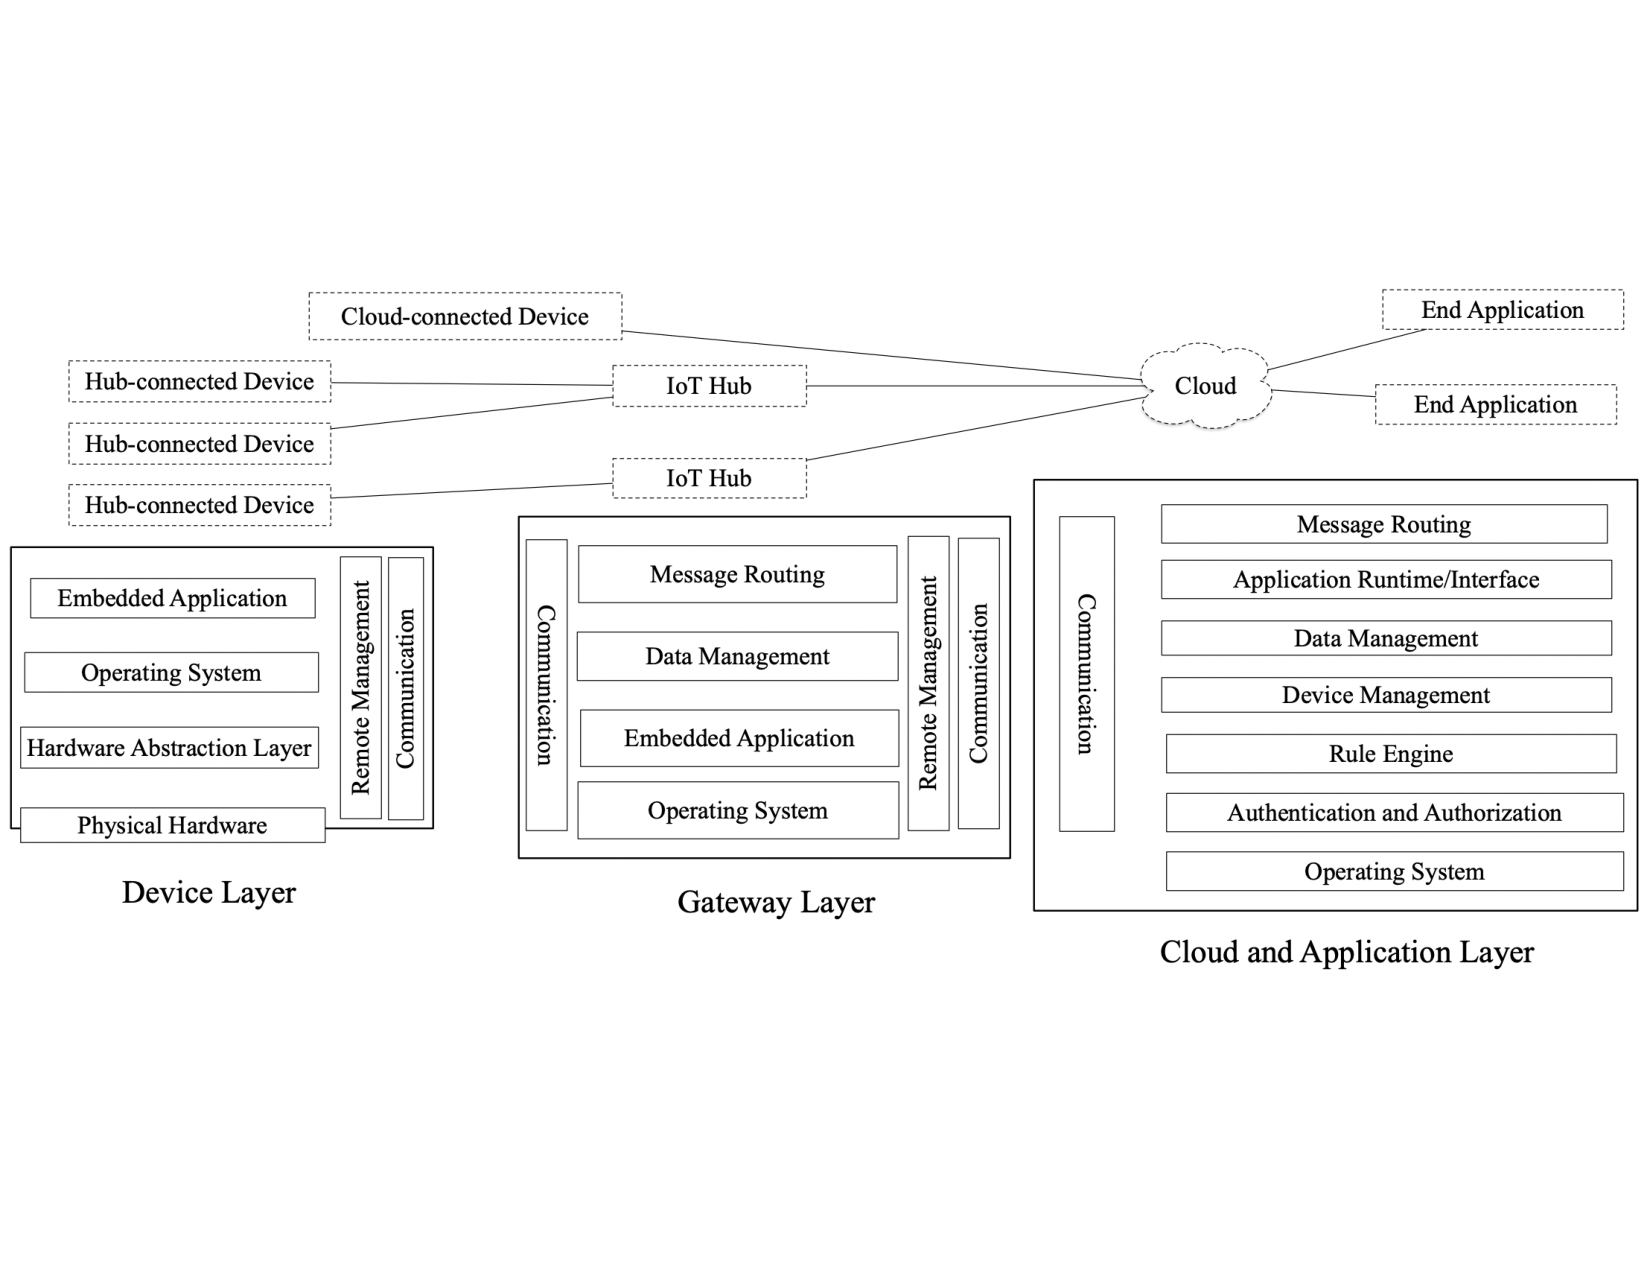
\includegraphics[width=\linewidth]{./imgs/arch1.pdf}
  \caption{A typical layered architecture of IoT systems and software stack for each layer}
  \label{fig:arch}
\end{figure}


\subsection{Gateway Layer}
This layer contains gateway devices with fewer resource constraints with the ability to handle telemetry data collection, processing, and routing locally on the edge. Gateway devices can handle the device-device and device-cloud interoperability by interpreting diverse communication protocols such as MQTT, CoAP, and HTTP~\cite{tschofenig2014architectural}. 

The IoT gateway devices have less resource constraint and the ability to handle telemetry data collection, processing, and routing locally on the edge. These devices can offer secure communication with remote systems since they can employ full-stack communication protocols and security mechanisms\cite{bormann2014terminology}.

There are different types of IoT devices based on their processing, power, and storage capabilities~\cite{bormann2014terminology} which affects the way they communicate with the cloud systems over the internet. Gateway-connected devices, as the name suggested in~\cite{securityUsenix2019}, are designed to do a limited functionality due to their constrained resources, thus, they rely on gateway devices for specific application purposes, data management, or secure communication with remote cloud systems~\cite{bormann2014terminology}. On the other hand, cloud-connected devices have the ability to talk directly to the cloud by employing protocols designed specifically for constrained devices like Constrained Application Protocol (CoAP). They should have enough resources to do basic data pre-processing and to apply security mechanisms by themselves without the help of a gateway device~\cite{stojkoska2017review,securityUsenix2019}. Gateway devices can handle the device-device and device-cloud interoperability by interpreting diverse communication protocols of both sides\cite{vcolakovic2018IoT}. Both types of IoT devices allow higher level components to control, monitor, and upgrade them remotely~\cite{eclipse2016three}.

\subsection{Cloud and Application Layer}
Remote IoT cloud servers accumulate and process all telemetry data, and communicate with a large number of heterogeneous gateway or cloud-connected devices to control and monitor them remotely. IoT cloud servers rule engine lets users write automation logic between IoT devices to define interoperability behaviours of the IoT system~\cite{securityUsenix2019}. 

End users and end applications can monitor the telemetry data and device status, and send commands to IoT devices to control and configure them remotely from the cloud. Usually, external end users and end applications should be authenticated and authorized in the cloud to be able to use these services. Some IoT cloud providers offer an interface for third-party applications, and allow users to run custom code in the application runtime environment on top of the cloud services\cite{vcolakovic2018IoT} and also allow them to have direct access to the analytical data via various visualizations and customized dashboards.


\section{Motivation}
\afterpage{%
 \begin{figure}[t]
  \centering 
   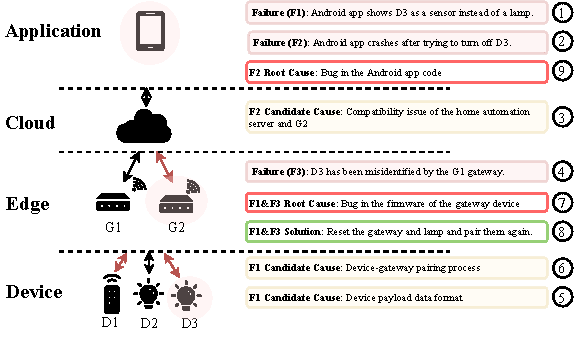
\includegraphics[width=\linewidth]{./imgs/motiv.pdf}
  \caption{The steps IoT developers have went through to find the root cause of a real IoT bug occurred in~\cite{iotbug:290}.}
  \label{fig:arch}
\end{figure}
\clearpage
}

Dealing with bugs and their causes in IoT systems is not a trivial task for developers. Below, we will do an in-depth investigation of a real bug report in an IoT system as an example of how dealing with bugs can be time-consuming for IoT developers. In addition to discussing the bug, we also showcase some challenges IoT developers have went through while debugging. 

Figure \ref{fig:arch} shows (on the right side) the steps that IoT developers have taken to find the root cause of the bug report PYTRADFRI/135~\cite{iotbug:290}. This bug occurred in a smart home environment where different devices should be connected to a home automation server with the help of a gateway device.


Based on developers' discussions, the first manifestation of this bug happens at the application layer. A light bulb device (D3) is mistakenly recognized as a sensor device (F\textsubscript{1}) as the user adds it, and also the Android app crashes (F\textsubscript{2}) once it tries to turn the light bulb off (step 1 and 2). Initially, the developers suspected the root cause of the bug to be the incompatibility of a gateway library with the home automation server (step 3).


However, further investigation of the failure in the edge layer (step 4), revealed that the gateway misidentifies D3 as a remote controller (F\textsubscript{3}). Since the gateway in this system relies mainly on a specific format of response data from devices to identify their types properly, potential inconsistencies of the payload data from the subject device were also investigated (step 5). In addition, developers should consider the device type, model, manufacturer, and the firmware version to detect possible breaking changes in the device firmware by the device manufacturer. 

But, further investigation eliminated the possibility of the device payload data as the root cause as some users reported that the same setting has not caused any issue for them. As the next step developers tried pairing in different circumstances (step 6), since the device battery and distance to the gateway could affect the pairing process. After none of the candidate causes showed as the potential reason for the bug, the root cause was identified as an external bug in the firmware of the G2 gateway device (step 7) and resetting both the device and the gateway and pairing them again solved the issue (step 8). But surprisingly F\textsubscript{2} continued to exist. After monitoring the data that the app receives via Wireshark, the root cause of F\textsubscript{2} was identified as a fault in the Android app code (step 9).

This example shows how one bug in the firmware of the gateway device, can make a lamp in the device layer useless, and cause observable failures in edge and application layers. Distribution of IoT failures and their candidate causes in different layers of IoT required a wide range of development skills from developers, as we could see that developers have to both investigate low-level firmware code and debug high-level application code to find the root cause of a single bug. Also dealing with behaviours of diverse devices such as comparing their payload, and depending on naive debugging practices such as monitoring network traffic, make it extremely hard for developers to deal with IoT bugs. Another challenging factor that we observed in this case study, is the interference of physical factors like the battery and the distance of the IoT devices from the gateway devices, which makes the debugging process rather time-consuming and complex.

Despite these compelling challenges, previous studies~\cite{hnat2011hitchhiker,corno2019challenges,stojkoska2017review,chen2017application,IoTOSBugs} do not take into consideration real-world experiences of IoT developers. In this paper, we aim to provide a systematic and generalized understanding of bugs and challenges in IoT by mainly considering IoT developers' experiences.

\endinput


%% The following is a directive for TeXShop to indicate the main file
%%!TEX root = diss.tex

\chapter{IoT Bugs}
\label{ch:bugs}

\section{Methodology}
Our goal from this study is to characterize software bugs in IoT systems. To this end, we address the following research questions in this study:
\begin{itemize}
\item {\verb|RQ1|}: What are the classes of bugs in IoT systems?
\item {\verb|RQ2|}: What are the root causes of IoT bugs?
\item {\verb|RQ3|}: What are the perceived severity and frequency of IoT bugs by real IoT developers?
\item {\verb|RQ4|}: What IoT bugs are more likely to happen together and have higher correlation?
\end{itemize}
In order to answer these questions, we conduct an empirical investigation consisting of two phases. In the first phase (RQ1), we analyze 323 issues and pull requests (PR) from open-source IoT projects. We use the findings to form the first taxonomy of bugs in IoT systems. In the second phase (RQ2), we conduct a qualitative study through (1) semi-structured interviews with IoT developers to discover new categories of bugs, (2) a survey of IoT developers to validate the findings about IoT bugs and gain new insights. All our quantitative and qualitative data is available online~\cite{repPack} 


 \begin{figure}
  \centering
   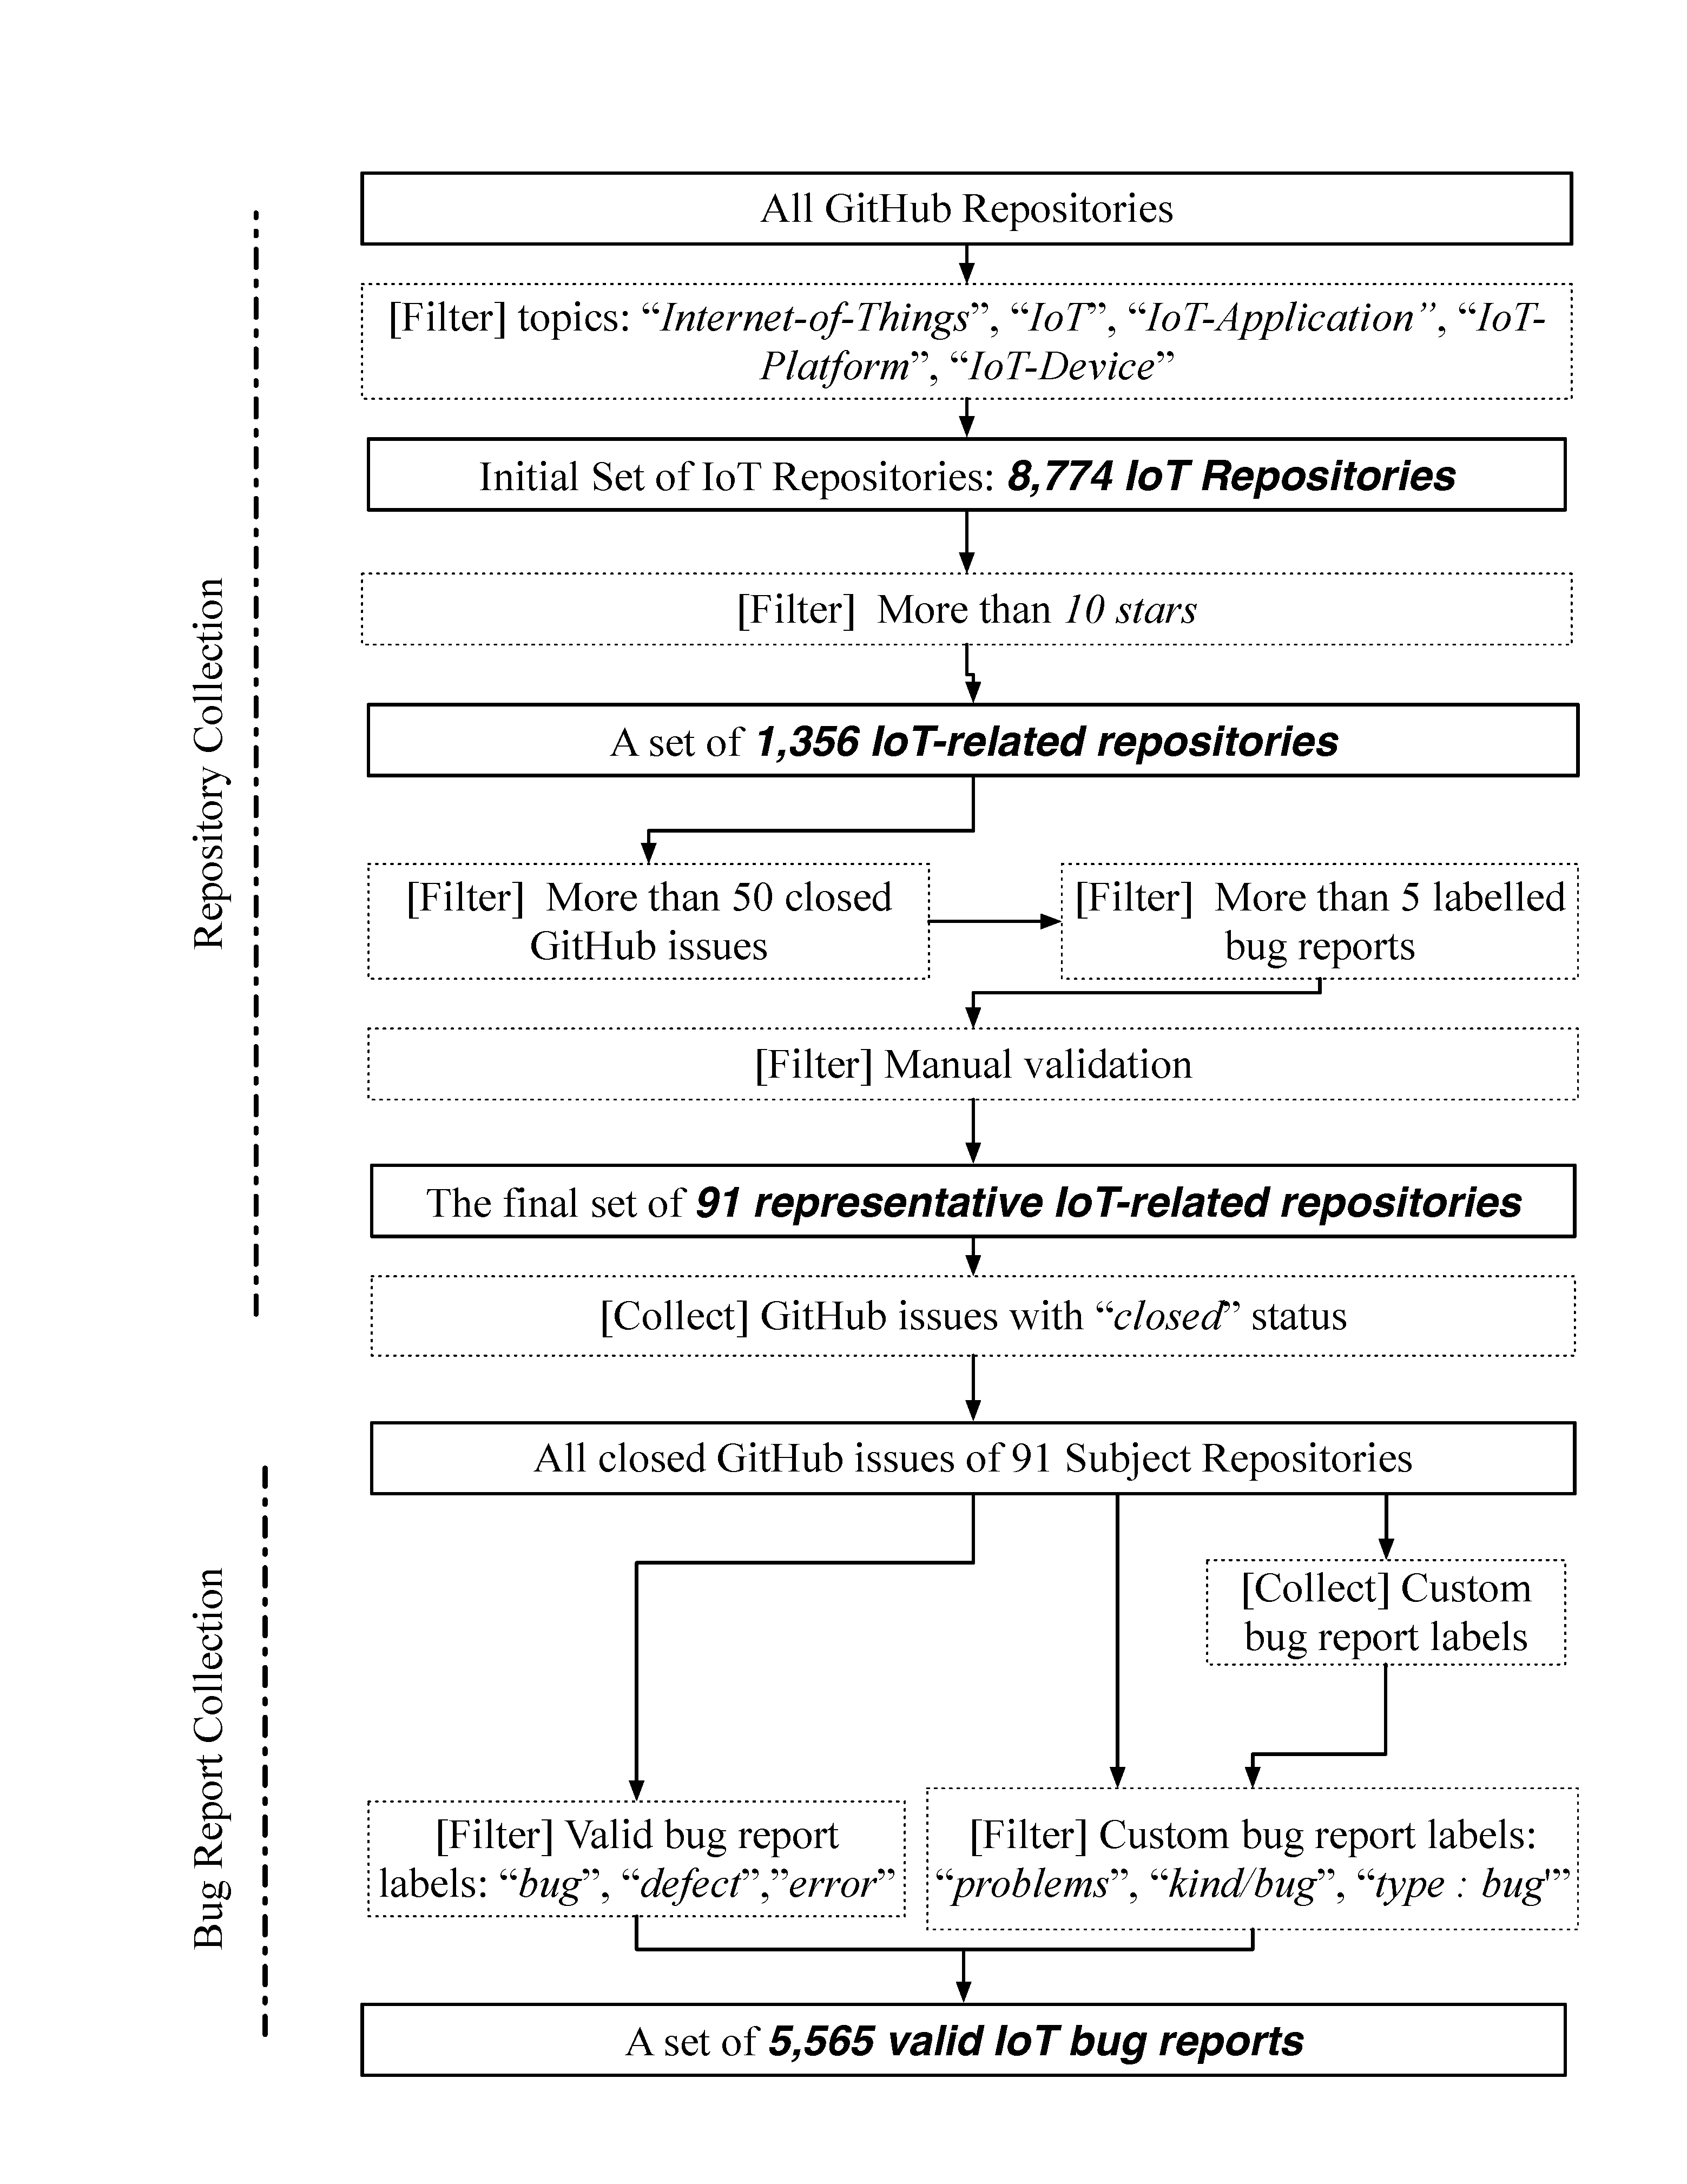
\includegraphics[width=\linewidth]{imgs/steps4repo.pdf}
  \caption{Our approach to collect subject IoT repositories and their valid bug reports.}
  \label{fig:steps4repo}
\end{figure}

\subsection{IoT Bug Categorization}
\subsubsection{Collecting bug reports} \label{bugCollection}

Figure \autoref{fig:steps4repo} shows the steps we took to find out subject IoT repositories and collect valid bug reports from them. The initial step is to find repositories that are representative of IoT projects. We employed the ``GitHub topic feature'' to find IoT-related repositories. According to GitHub's official website~\cite{gitTopic}, Topics are labels that create subject-based connections between GitHub repositories. Repository owners can use multiple tags for their repository to help users in exploring projects based on their technology, subject area, or domain.

 We searched among topics with related keywords such as "internet-of-things" and "IoT" and we added the top three topics ``IoT-application'', ``IoT-platform'', and ``IoT-device'' from the results to our list of targeted topics. Initially, we collected 8,774 repositories using these five topics in January 2020. Inspecting a random sample of 30 repositories showed that 86\% of them have less than 5 issued bug reports, while 50\% of them did not have a single bug report. A previous study~\cite{borges2018s} found that 3 out of 4 developers check the stars metric before using or contributing to a GitHub project. 
Thus, In order to reduce the number of GitHub API requests, we excluded repositories with less than 10 stars~\cite{borges2018s}, resulting in 1,356 repositories to consider.

To only consider valid bugs, we looked for issued bug reports with only ``closed'' status and with ``bug''', ``defect'', or ``error'' labels.  Moreover, to select only representative IoT repositories for our study, we manually analyzed repositories that have more than five labeled issues or more than 50 closed issues based on the information in their readme page, issued bug reports, and their website (when available). We then excluded projects that were not representative of IoT systems such as user interface, documentation, or outdated repositories. Our final project list contained 91 open source IoT repositories to analyze. For five repositories that use custom labels (e.g., ``problems'', ``kind/bug'', ``type : bug''), we manually added their labels to our search keywords. In the end, we collected \emph{5,565 bug reports} from the 91 IoT repositories.

Figure \autoref{fig:repodemog} shows the demographics of our subject repositories. The selected IoT repositories together cover all the layers of the IoT systems' architecture depicted in \autoref{fig:arch}. The most popular programming languages among the subject repositories are Python (21\%), Java (18\%), JavaScript (17\%), C (13\%), and C++ (13\%). A few of them use other programming languages such as Go, Ruby, and C\#. The selected repositories are also diverse in terms of the number of stars and forks they have. In February of 2020, 32\% of our subject GitHub repositories had more than 500 stars, 40\% between 50 to 500 stars, and 28\% between 10 to 50 stars.


 \begin{figure}
  \centering
   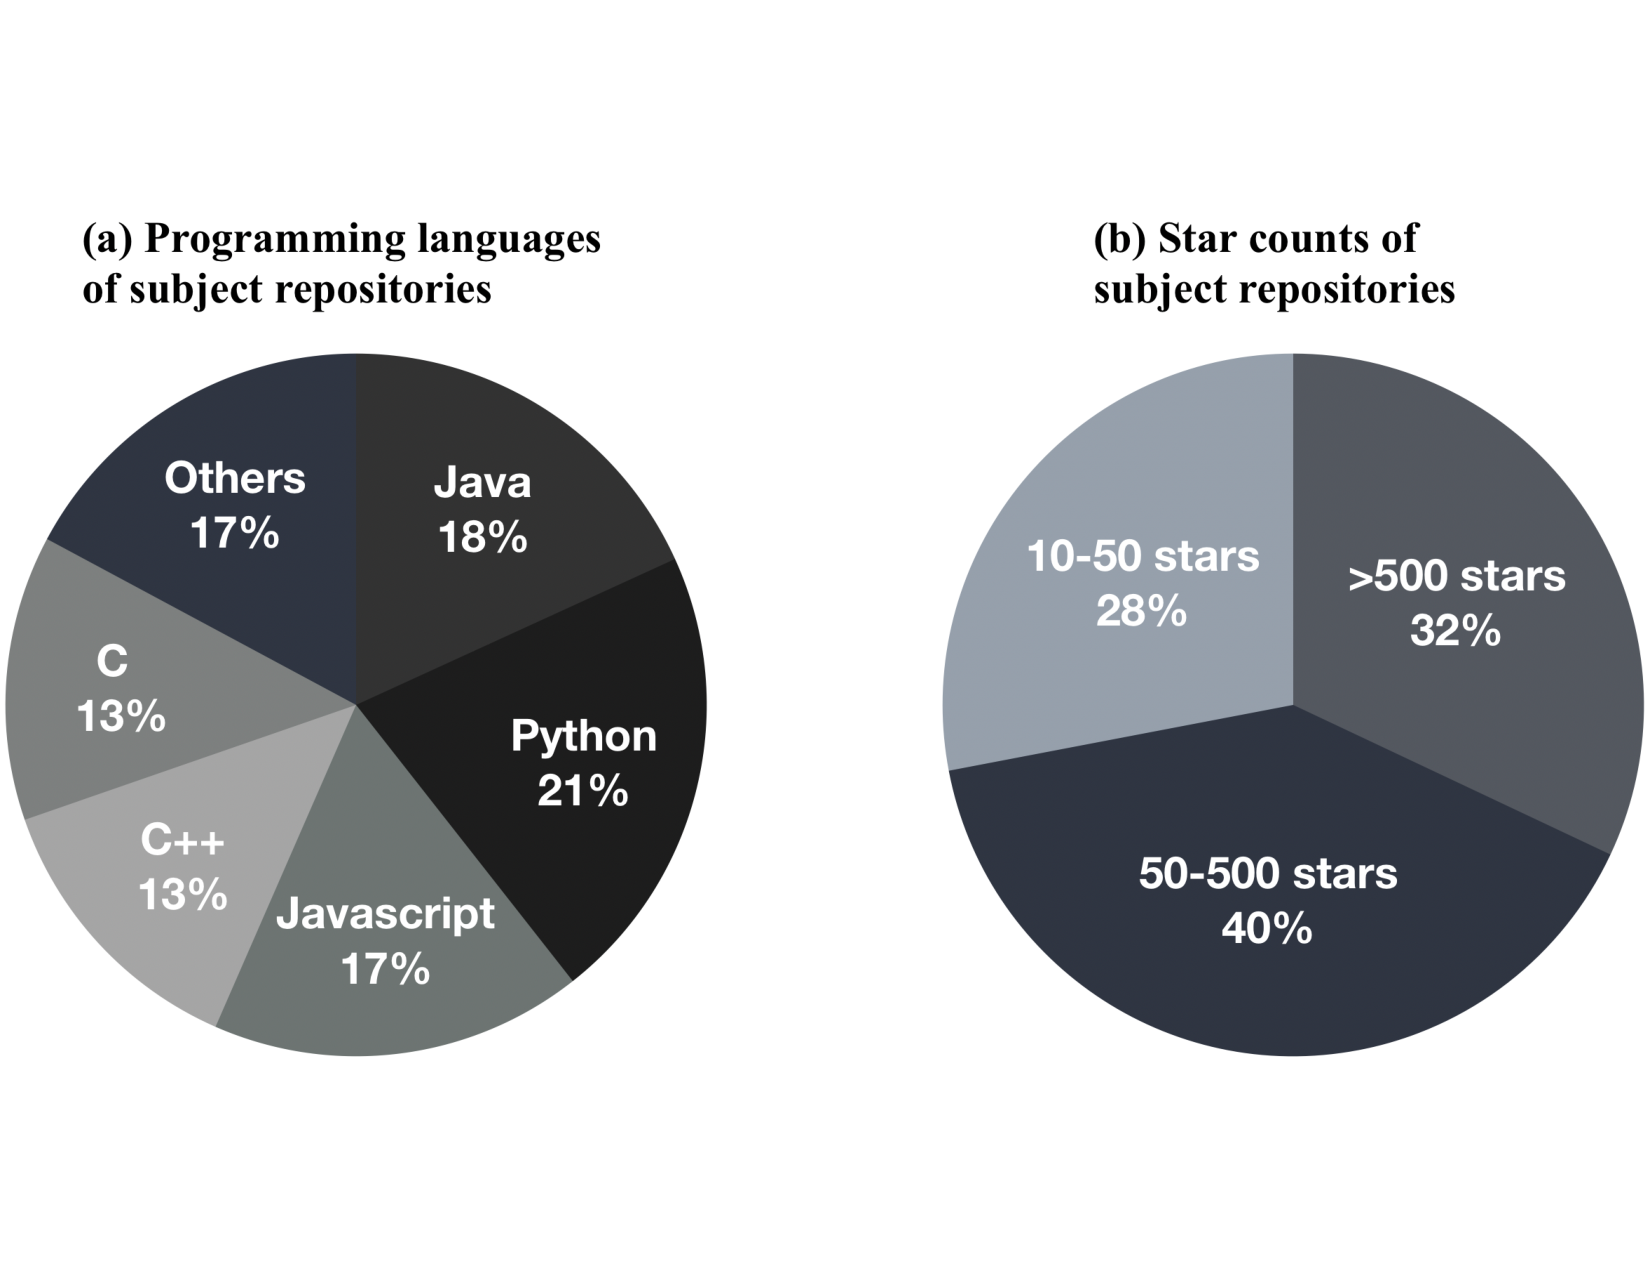
\includegraphics[width=\linewidth]{imgs/repodemog}
  \caption{(a) Programming languages of subject repositories and (b) their star count.}
  \label{fig:repodemog}
\end{figure}


\subsubsection{Labeling} 
Figure \autoref{fig:labeling} shows the steps we took to label bug reports. For each bug report in our dataset, we created a JSON object containing failure(s), cause(s) of the failure, and location(s) of the faulty code. Failure refers to any observable unexpected behavior of the system that is against the correct functionality of that system~\cite{bugCharOpenSoftware,failureDefinition}. To explore the causes of the failure, we did RCA on each bug report using the \emph{five whys technique}~\cite{serrat2017five}. Based on this technique, multiple causes can contribute together or at different levels to a visible failure in the system. Following this approach, we started from the failure and repeatedly asked ``why'' until we reached the root cause of the problem. In the case of software failures, root causes are often developers' faults in the design or implementation of the IoT system. To label the location(s) of faults, we used the architecture defined in Chapter \ref{ch:background} as our reference. 

Bug reports were manually labeled by the author(s) individually following the open coding procedure~\cite{qualitativeStudySE}. We followed an iterative process for labeling where in each iteration, we randomly sampled new instances from the collected bug reports and labeled them. After each labeling iteration, all potential conflicts in labels between the author(s) were resolved. We continued this process until bug categories reached a state of saturation where no new category appeared~\cite{dataSaturationFusch}. 

We also flagged and discarded issues and PRs that could not represent a bug or a bug-fix such as enhancements or how-to-use questions. We examined the entire discussion among developers, as well as the fix commit data (e.g. the commit message and the code diff) to label each bug report. At the end, we labeled \emph{323 bug reports}.

 \begin{figure}
  \centering
   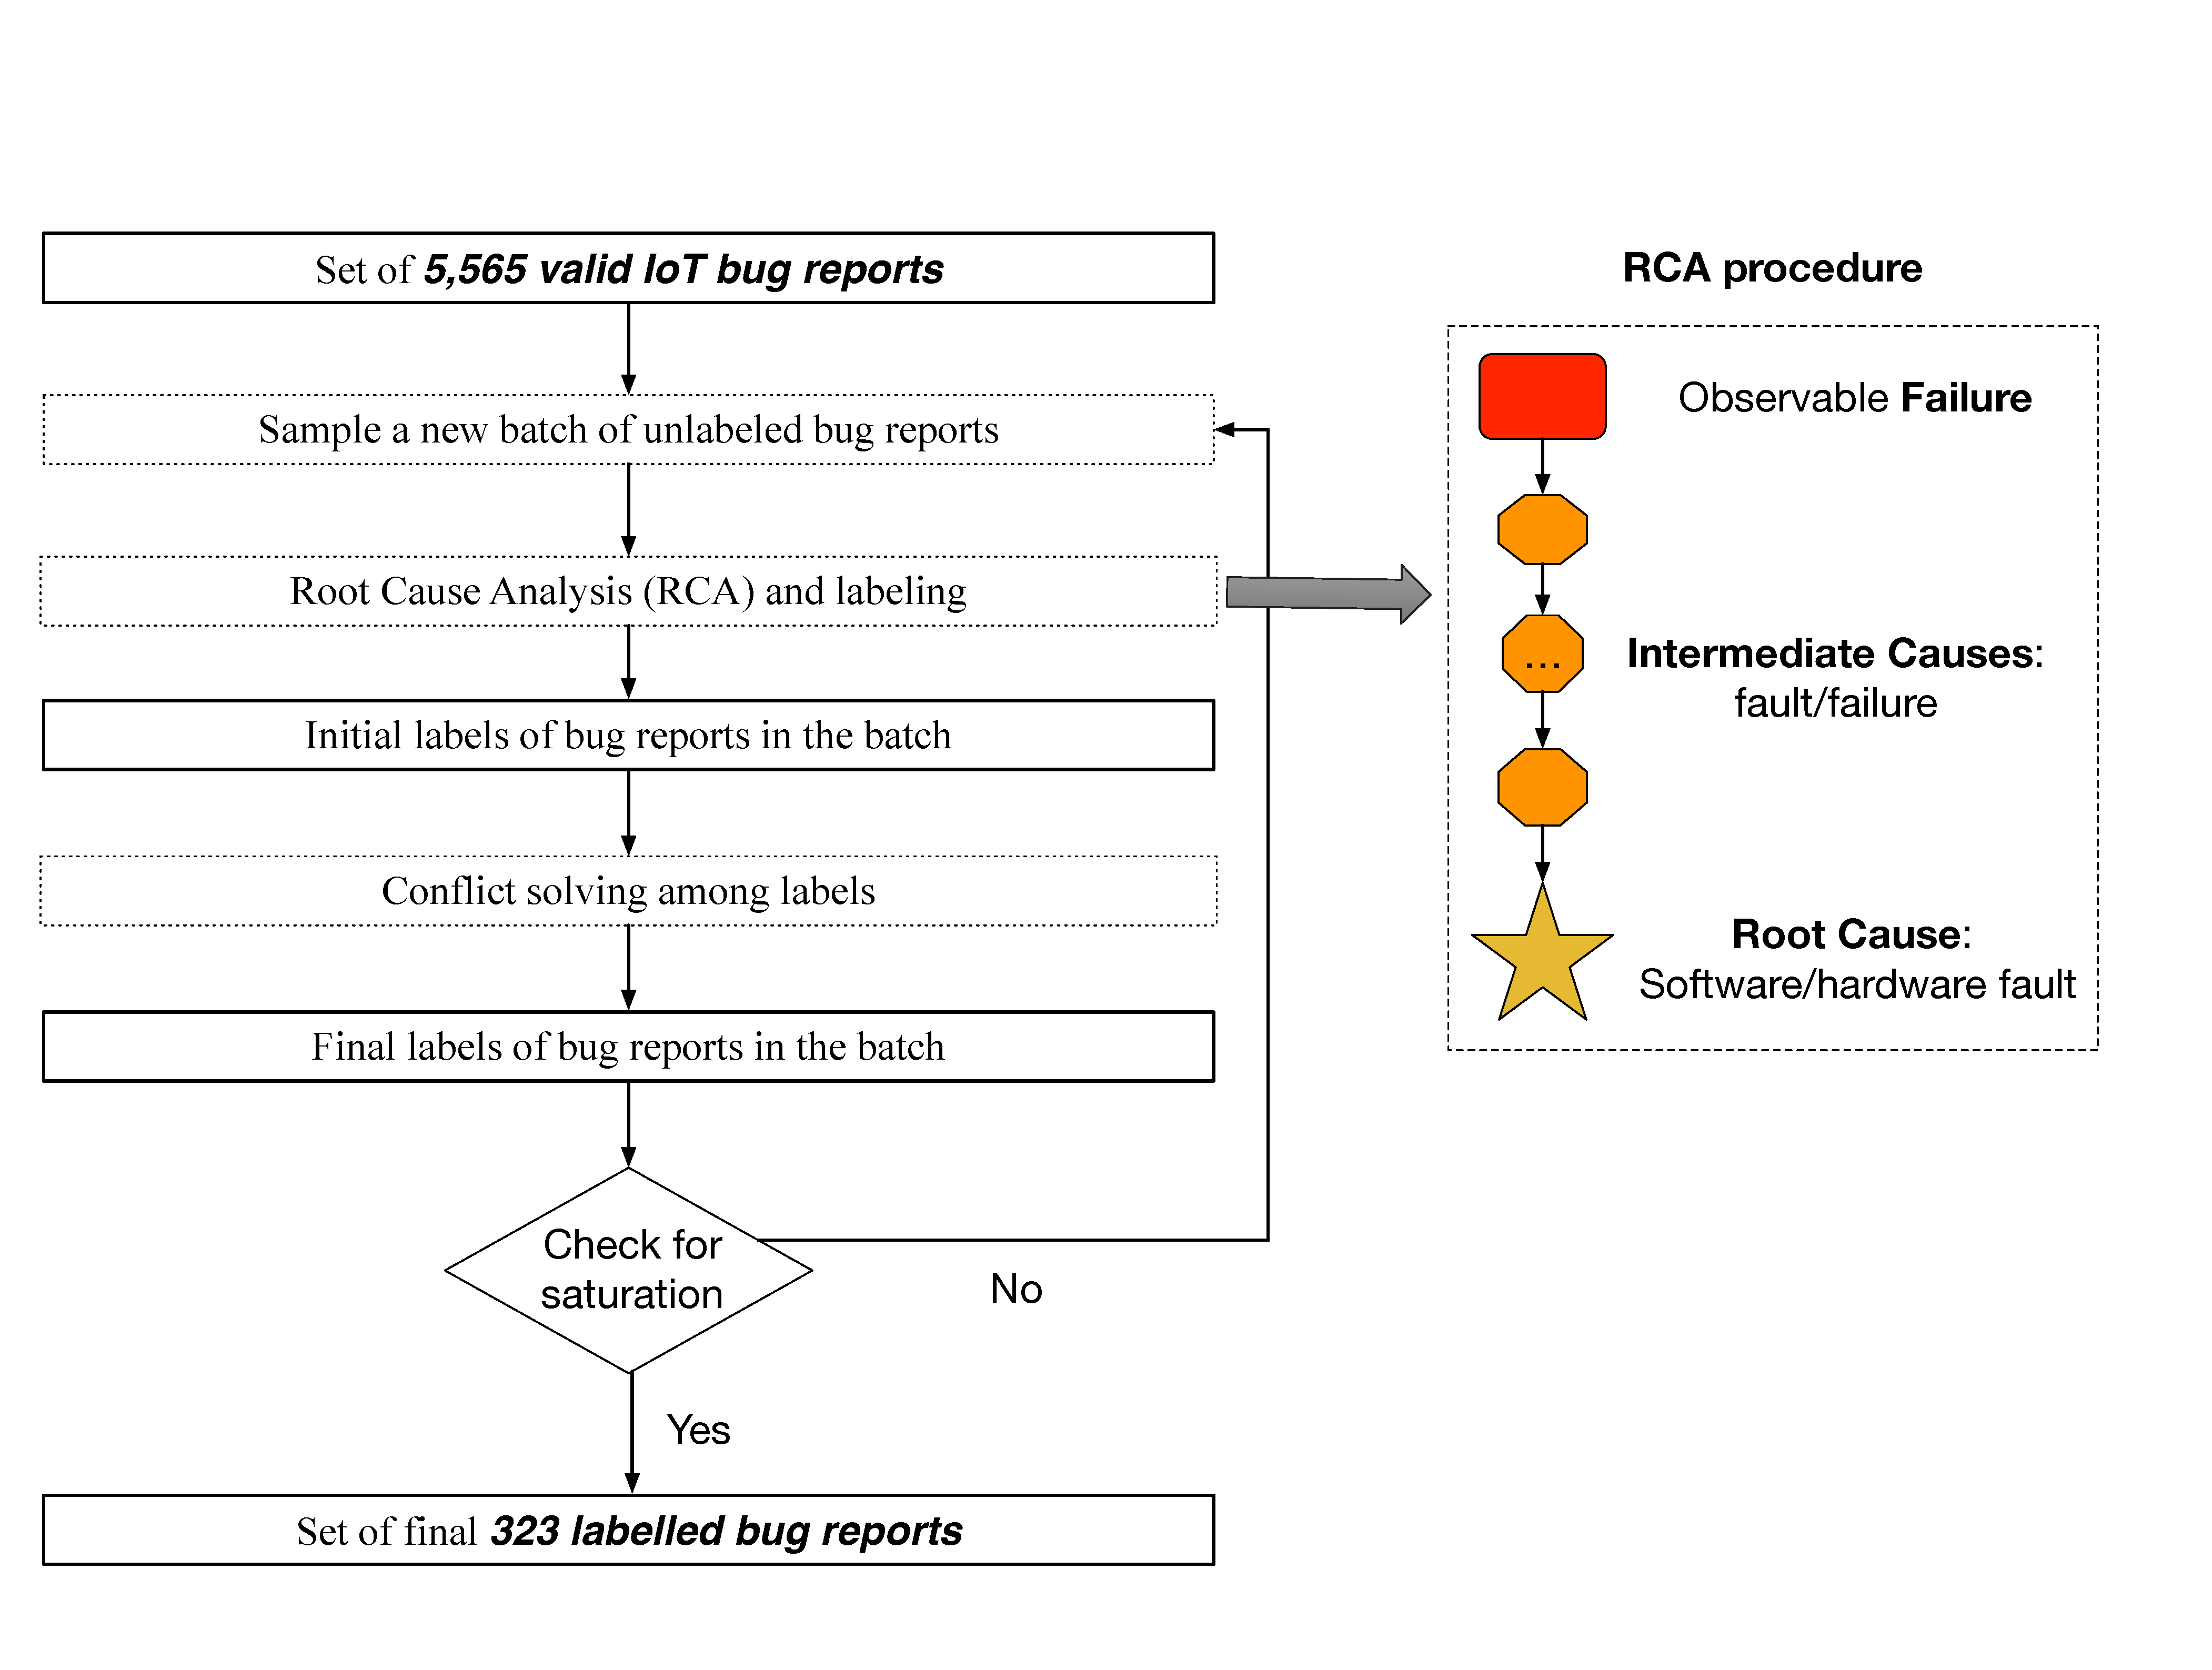
\includegraphics[width=\linewidth]{imgs/labeling}
  \caption{(a) Programming languages of subject repositories and (b) their star count.}
  \label{fig:labeling}
\end{figure}

\begin{table}[htbp]
\caption{Interview Participants}
\resizebox{\linewidth}{!}{%
\begin{tabular}{c l l l r r}
\hline
\textbf{ID}& \textbf{Role }&\textbf{IoT Systems Type}& \textbf{Projects Domain}  & \textbf{Dev Exp (yr)} & \textbf{IoT Dev Exp (yr)}  \\
\hline
P1 &  Software and hardware lead & Full-stack & Smart home  & 13  & 7   \\
P2 & Hardware lead & Hardware & Education& 15  & 5    \\
P3 & Software dev & Full-stack & Smart home & 5  & 4   \\
P4 & Software dev & Middleware & Smart city & 3  & 3    \\
P5 & Software lead & Full-stack & Smart home & 20  & 17   \\
P6 & Software dev  & Cloud &  Not domain-specific & 10  & 3 \\
P7 & Software and hardware dev & Full-stack & Smart home & 20  & 3   \\
P8 & Software lead  & Full-stack & Smart home & 11  & 4  \\
P9 & Software lead  & Cloud & Not domain-specific & 20  & 12  \\
\hline
\end{tabular} }
\label{tab1}
\end{table}

\subsection{Interviews} \label{interviews4Bug}
 While manual analysis of bug reports and developers' discussions provided useful insights into the characteristics of IoT development, there was still a possibility that our bug categories are not generalizable. To mitigate this issue, we conducted semi-structured interviews with IoT developers to reveal new bug categories to complement and validate our results. 

\textbf{Participants} 

To collect interview participants, we employed GitHub as it provides a diverse pool of developers and their contributions to different projects.

To collect candidate interview participants, we followed the steps shown in figure~\autoref{fig:candidates}. We used the 1,356 IoT repositories we collected in section~\autoref{ bugCollection}, as the IoT projects with more than 10 stars, to sample interview participants. After collecting all the 11,129 contributors to these 1356 repositories, we removed duplicate contributors, resulting in 6,878 contributors. Duplicate contributors are the IoT developers involved in more than one repository from the set of subject repositories and thus appeared more than once in our initial dataset. The next step is to find the valid email addresses of these unique contributors.


GitHub API does not provide the email addresses of the developers directly. We searched through the information returned by GitHub public API from the requests regarding contributors' commits to extract their email addresses. This was the only way we could find to extract the email addresses of contributors to IoT repositories.  A manual run of this method showed that the email addresses of a handful of the contributors are unavailable or invalid. First of all, we removed the contributors that their email address has not appeared in any of the GitHub API's responses since our goal was to contact developers only via their email addresses. Moreover, we removed the contributors that their email address contains the string "no-reply" and its invariants. After all the filtering, we could obtain the valid email addresses of 1,847 unique contributors to popular IoT repositories.

For interviews, we only added the top three contributors to the set of candidate interviewers. We used purposive sampling~\cite{sampling2007} to recruit developers with adequate experience in developing IoT systems.  

We contacted candidates through emails and conducted interviews until we reached data saturation, where we had sufficient data to replicate the study and further data collection is unnecessary~\cite{dataSaturationFusch}. We relied on this widely-applied methodological principle to decide when to stop interviewing~\cite{saturationMorse,saturationGuest} as it is also used in other qualitative studies in software engineering~\cite{tweeter2014, aniche2018modern}. We interviewed people with different development backgrounds and experiences before deciding about the data saturation to consider variability in experimental results across different populations~\cite{henrich2010weirdest}. 


 Table \ref{tab1} presents all nine interview participant's experience and field of expertise in IoT development. For a high-level picture of their general development background, the lowest value is three years and the highest value is 20 years (avg=13, sdv=6.4). In terms of IoT development experience, the lowest value is three years and the highest value is 17 years (avg=6.4, sdv=4.6). Participants' IoT development experience covers all sections of IoT systems spanning from hardware to middleware, cloud, and end-applications. In addition, their projects cover a variety of domains such as smart home and Industrial IoT (IIoT). 

\afterpage{%
 \begin{figure}
  \centering
   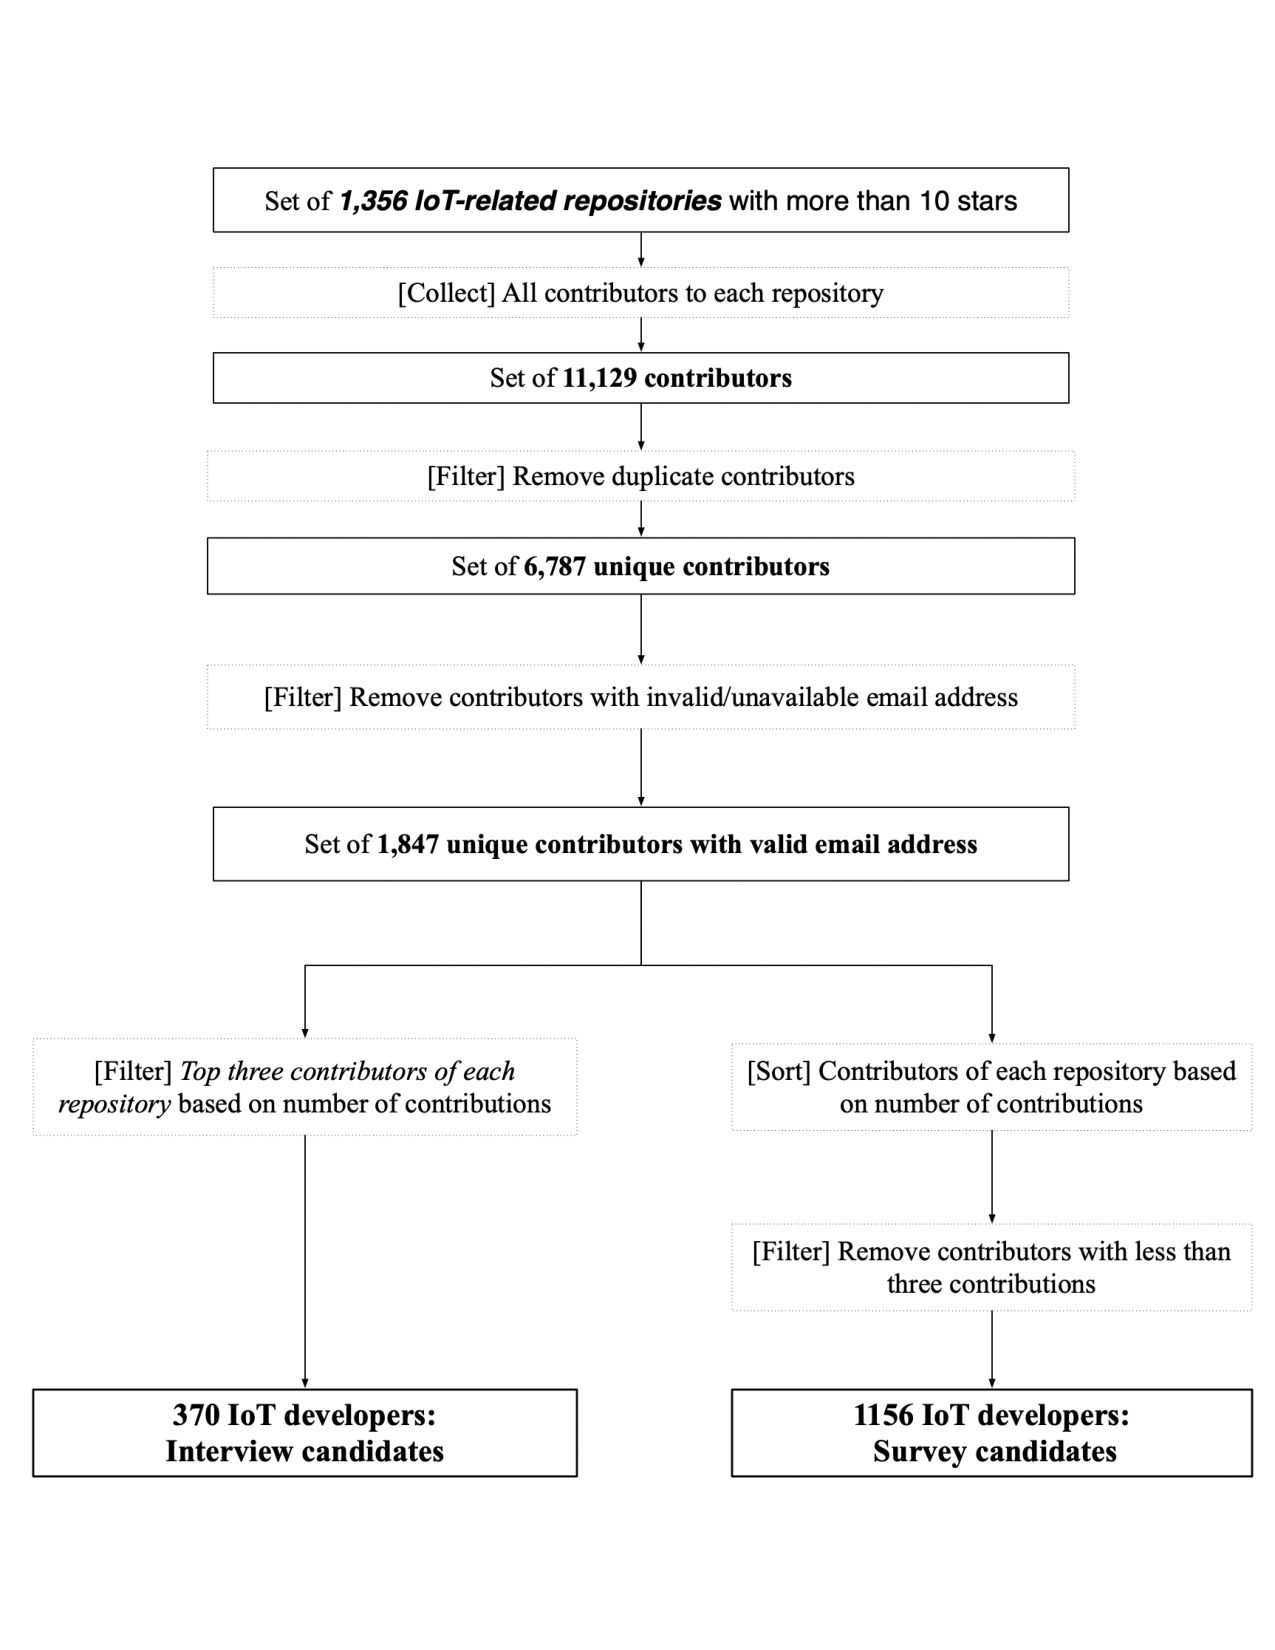
\includegraphics[width=\linewidth]{imgs/candidates.pdf}
  \caption{Our methodology for finding candidates for interviews and survey.}
  \label{fig:candidates}
\end{figure}
\clearpage
}

\textbf{Protocol} \label{interviewProtocol}
Since our goal for conducting interviews was to be open to new data, and we did not have the definitive structure of bug categories, we conducted interviews following a semi-structured approach. Interviews started with some questions about participants' IoT development background and their field of expertise in IoT. This information could help us improvising insightful questions during the technical section of the interviews. The technical section had a combination of both open-ended and specific questions about different categories of bugs and challenges in IoT development. Our strategy was to start with open-ended questions to avoid biasing participants toward our findings, and then we gradually shifted to more structured and predefined questions during the interview process.  With participants' consent, we recorded the audio and video of all the interviews for later analysis. All the interviews were conducted remotely through Zoom. Interviews took around 43 minutes on average ranging from 31--70 minutes. We used Descript, an automated speech detection tool, to generate transcribes of the interviews and we did manual corrections afterward in case of any mistakes in the automatically generated transcripts.

\textbf{Analysis} \label{interviewAnalysis}
As the primary objective of this study is to generate theories from the experiences of IoT practitioners instead of using pre-conceived theories, we followed the grounded theory methodology~\cite{grounded2007} to ensure the quality of the generated theory. Our analysis steps consist of iteratively (i) collecting qualitative data from the interviews (ii)  analyzing the interview transcript line by line and assigning labels (tags) to distinct units of meanings, and (iii) identifying emerging categories and relating categories to their subcategories while continuously comparing all the previously analyzed data with the emerging theories. These steps were repeated for each interview. On average, we extracted 18 tags per interview. Potential conflicts in the labels were resolved after each iteration by the authors. 

\subsection{Validation Survey} \label{survey4bug}
In order to make sure that our findings are generalizable, comprehensive, and representative, we involved more IoT developers through an online survey. 

\textbf{Participants} 
Figure~\autoref{fig:candidates} shows how we collected the survey participant candidates. Firstly, we sorted the collected unique contributors with valid email addresses based on the number of contributions they had to the 1,356 subject IoT projects. After removing the contributors with less than three contributions, we started to send out our survey to the resulting candidate participants until we reached saturation in our results. We gave higher priority to the developers with more contributions by sending our survey first to the developers with higher contributions.

We also sent out our survey to the IoT developer groups in social media platforms such as Linkedin and Facebook, and online forums. Our survey was online between 19 July and 19 August 2020. The survey, as distributed to participants, is available in our artifact package~\cite{repPack}.
 \begin{figure}
  \centering
   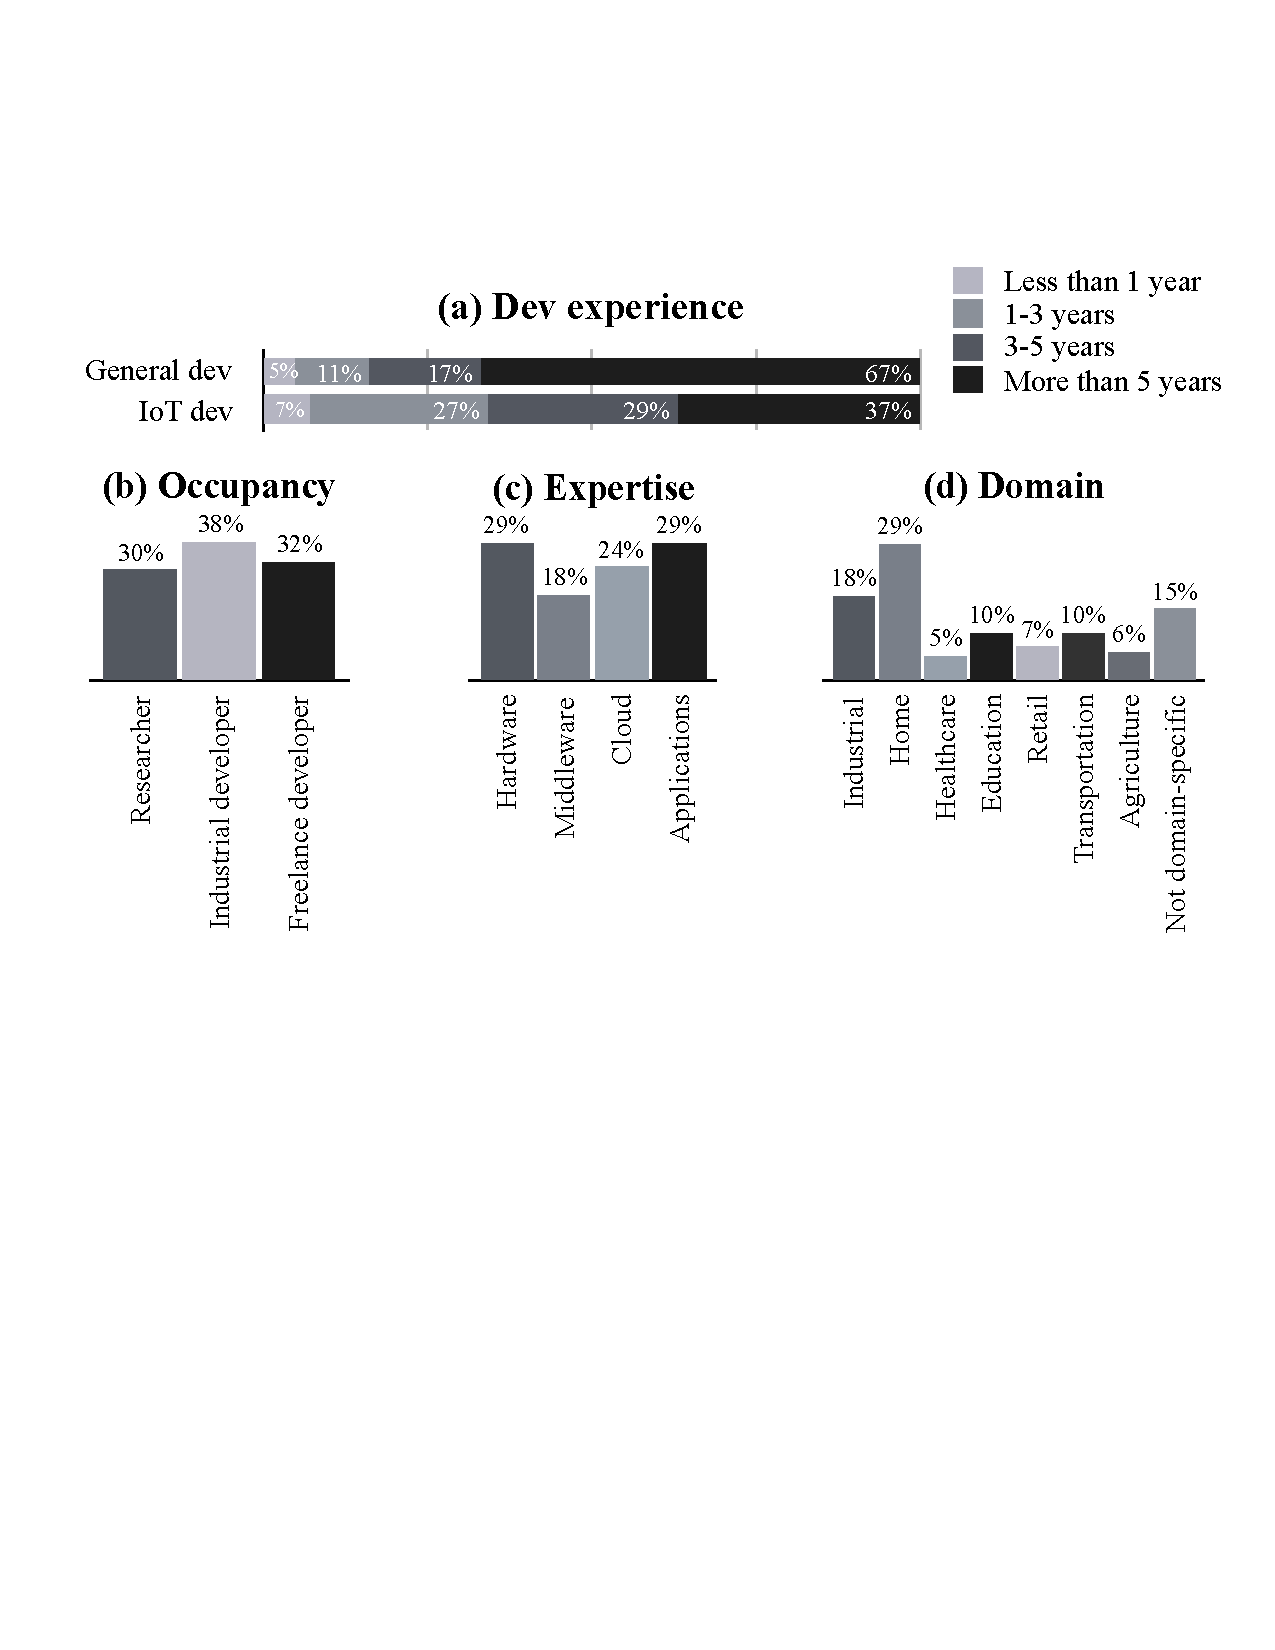
\includegraphics[width=\linewidth]{imgs/demog.pdf}
  \caption{Development backgrounds of the survey participants}
  \label{fig:demog}
\end{figure}

\textbf{Protocol}
The survey has three sections. In the first section, we collect participants' background in IoT, and in general development, which is depicted in~\autoref{fig:demog}. The second section concerns the challenges of developing IoT systems with questions aimed at correlating our findings with the participants' own experiences. 

The third section is about the frequency and severity of bug categories based on participants' previous experience in IoT development. At the end of each section, there are open-ended questions to allow them to share their comments about our results and mention new categories.

\textbf{Analysis}
Our survey was completed by 194 respondents, with a response rate of around 10\% for valid responses. 
 We received 95 comments through the open-ended questions sections. All of the survey respondents' comments are coded and analyzed following the same procedure discussed in \autoref{interviewAnalysis}.

\section{Findings: IoT Bug Categories (RQ1)}
In this section, we describe our findings regarding IoT bugs. 


\subsection{Taxonomy of Bugs}
We used all the tags collected by RCA of the bug reports in our dataset, to build a taxonomy of bugs in IoT systems. As our motivating example illustrates~\autoref{motivExample}, IoT bugs can be multi-faceted and manifest at different layers and locations. Therefore, we designed our bug taxonomy to accommodate all these bug characteristics. Considering various approaches suggested by Usma et. al.~\cite{usman2017taxonomies} for taxonomy construction, we followed the approach suggested by Kwasnik~\cite{kwasnik1999role} as IoT bugs are multi-faceted and relatively a new and unexplored concept. Following their approach, we first defined facets of our classification as all failures and locations of failures. Then, we analyzed all bug reports based on these facets and built a hierarchical taxonomy that accommodates all the dimensions.

After we built the initial version of the taxonomy, we used the data from the interviews and the survey to complement and enhance the taxonomy. We reviewed all previously tagged data and re-tagged them after each alteration of the taxonomy. \autoref{bugTax} depicts our IoT bug taxonomy. Next, we describe the major bug categories in our taxonomy. We will use specific bugs as examples for each category. All these bug examples are available in our dataset, which is available online~\cite{repPack}. 


\textbf{IoT Device}
This category of taxonomy covers bugs that are related to IoT device hardware and firmware.

\textit{Device hardware:}
Bugs in this subcategory are related to the physical aspects of IoT devices.  Examples include bugs related to wiring issues, device pin status issues, or issues with physical sensors and actuators of the device. For example, PEDALINOMINI/34 is related to the device not differentiating between single and double presses of a hardware button. 
 
 Other common bugs in this category are those that are linked to the device's limitations in memory, power consumption, or processing capacity. One such instance provided by P\textsubscript{1} as he described a scenario where a device on low battery generated incorrect data to the cloud. There are various similar cases in our collected bug reports where the low battery of the device or the removal of the power source of the device causes failures. Even in some cases, enabling power saving mode cause unexpected behaviours such as variable lag. For example, in DEVICE-OS/1567, the power saving mode causes some variable lag, which led IoT developers to disable the power saving mode as they had not accounted for such delays.
 
 Another group of device hardware issues is the problems regarding booting or rebooting the device. For example, heavy calculations and processing on the device (HOMIE-ESP8266/575, interviewee P\textsubscript{8}) cause a device boot loop issue. Also, there are cases where the IoT device runs out of memory (ZWAVE2MQTT/141, interviewee P\textsubscript{7}) which are other types of bugs related to this category. Another example of known hardware issues of IoT devices is the known timing issues of Raspberry Pi devices~\cite{piClockissues},  which is also mentioned by an interviewee (P\textsubscript{8}).

\textit{Device firmware:} 
Firmware bugs consist of three subcategories. The first pertains to device firmware unexpected exception and hang issues. The second sub-category includes issues related to the configuration of the IoT device, which can be specified as an external instruction sent to the device for a specific purpose. This type of bug usually happens in the early stages of introducing an IoT device to the IoT network. Each device has to be configured properly in a way to be compatible with other hardware or software components and also be able to communicate with others on the network. Issues associated with configuring the device with WiFi credentials or with configuring the device with the correct firmware version are some common examples here. The third and most common sub-category is the firmware upgrade issue. There are various cases where poor practices for handling over-the-air (OTA) updates of the device firmware, stale updates, or updating the device firmware with the wrong binary have caused failures of the IoT system.
In some cases, the stale update issues are related to device configuration issues as in WTHERMOSTATBECA/54, where the device needs to be re-configured with WiFi credentials after each firmware update, otherwise, future firmware updates would be stale. 

\textbf{Compatibility}
When a bug occurs only on a specific type of device, communication protocol, or third-party component, it falls under the compatibility category. For instance, a common device incompatibility issue happens when certain devices represent their telemetry data in different formats, leading to the other components not being able to process their data. Other common bugs are linked to compatibility issues of certain combinations of sensors and development boards, e.g., incompatibility of the DHT temperature sensor with the ESP32 microcontroller in MONGOOSE-OS/277. Issues with the interoperability of different protocols is another case. One example is MAINFLUX/1079, which is related to the interoperability between the HTTP and MQTT protocols. A common bad practice in IoT development related to these issues is developing protocol-specific or device-specific code. For instance, in DEVICE-OS/1938, the IoT platform relies on event components to report what protocols each event is intended for, in order to be able to run different functions for each protocol individually. However, sometimes developers have no other choice but to follow this error-prone approach, just to bypass the limitations of third-party devices. For instance, (P\textsubscript{2}) mentioned a case where the incompatibility of the Raspberry Pi and some types of sensors had forced their developers to implement custom logic for the communication of these devices. Developers had to switch between Raspberry Pi's default implementation and their own custom implementation based on the sensor type, leading to many issues.

\afterpage{%
\begin{figure*}%[ht]
  \centering
   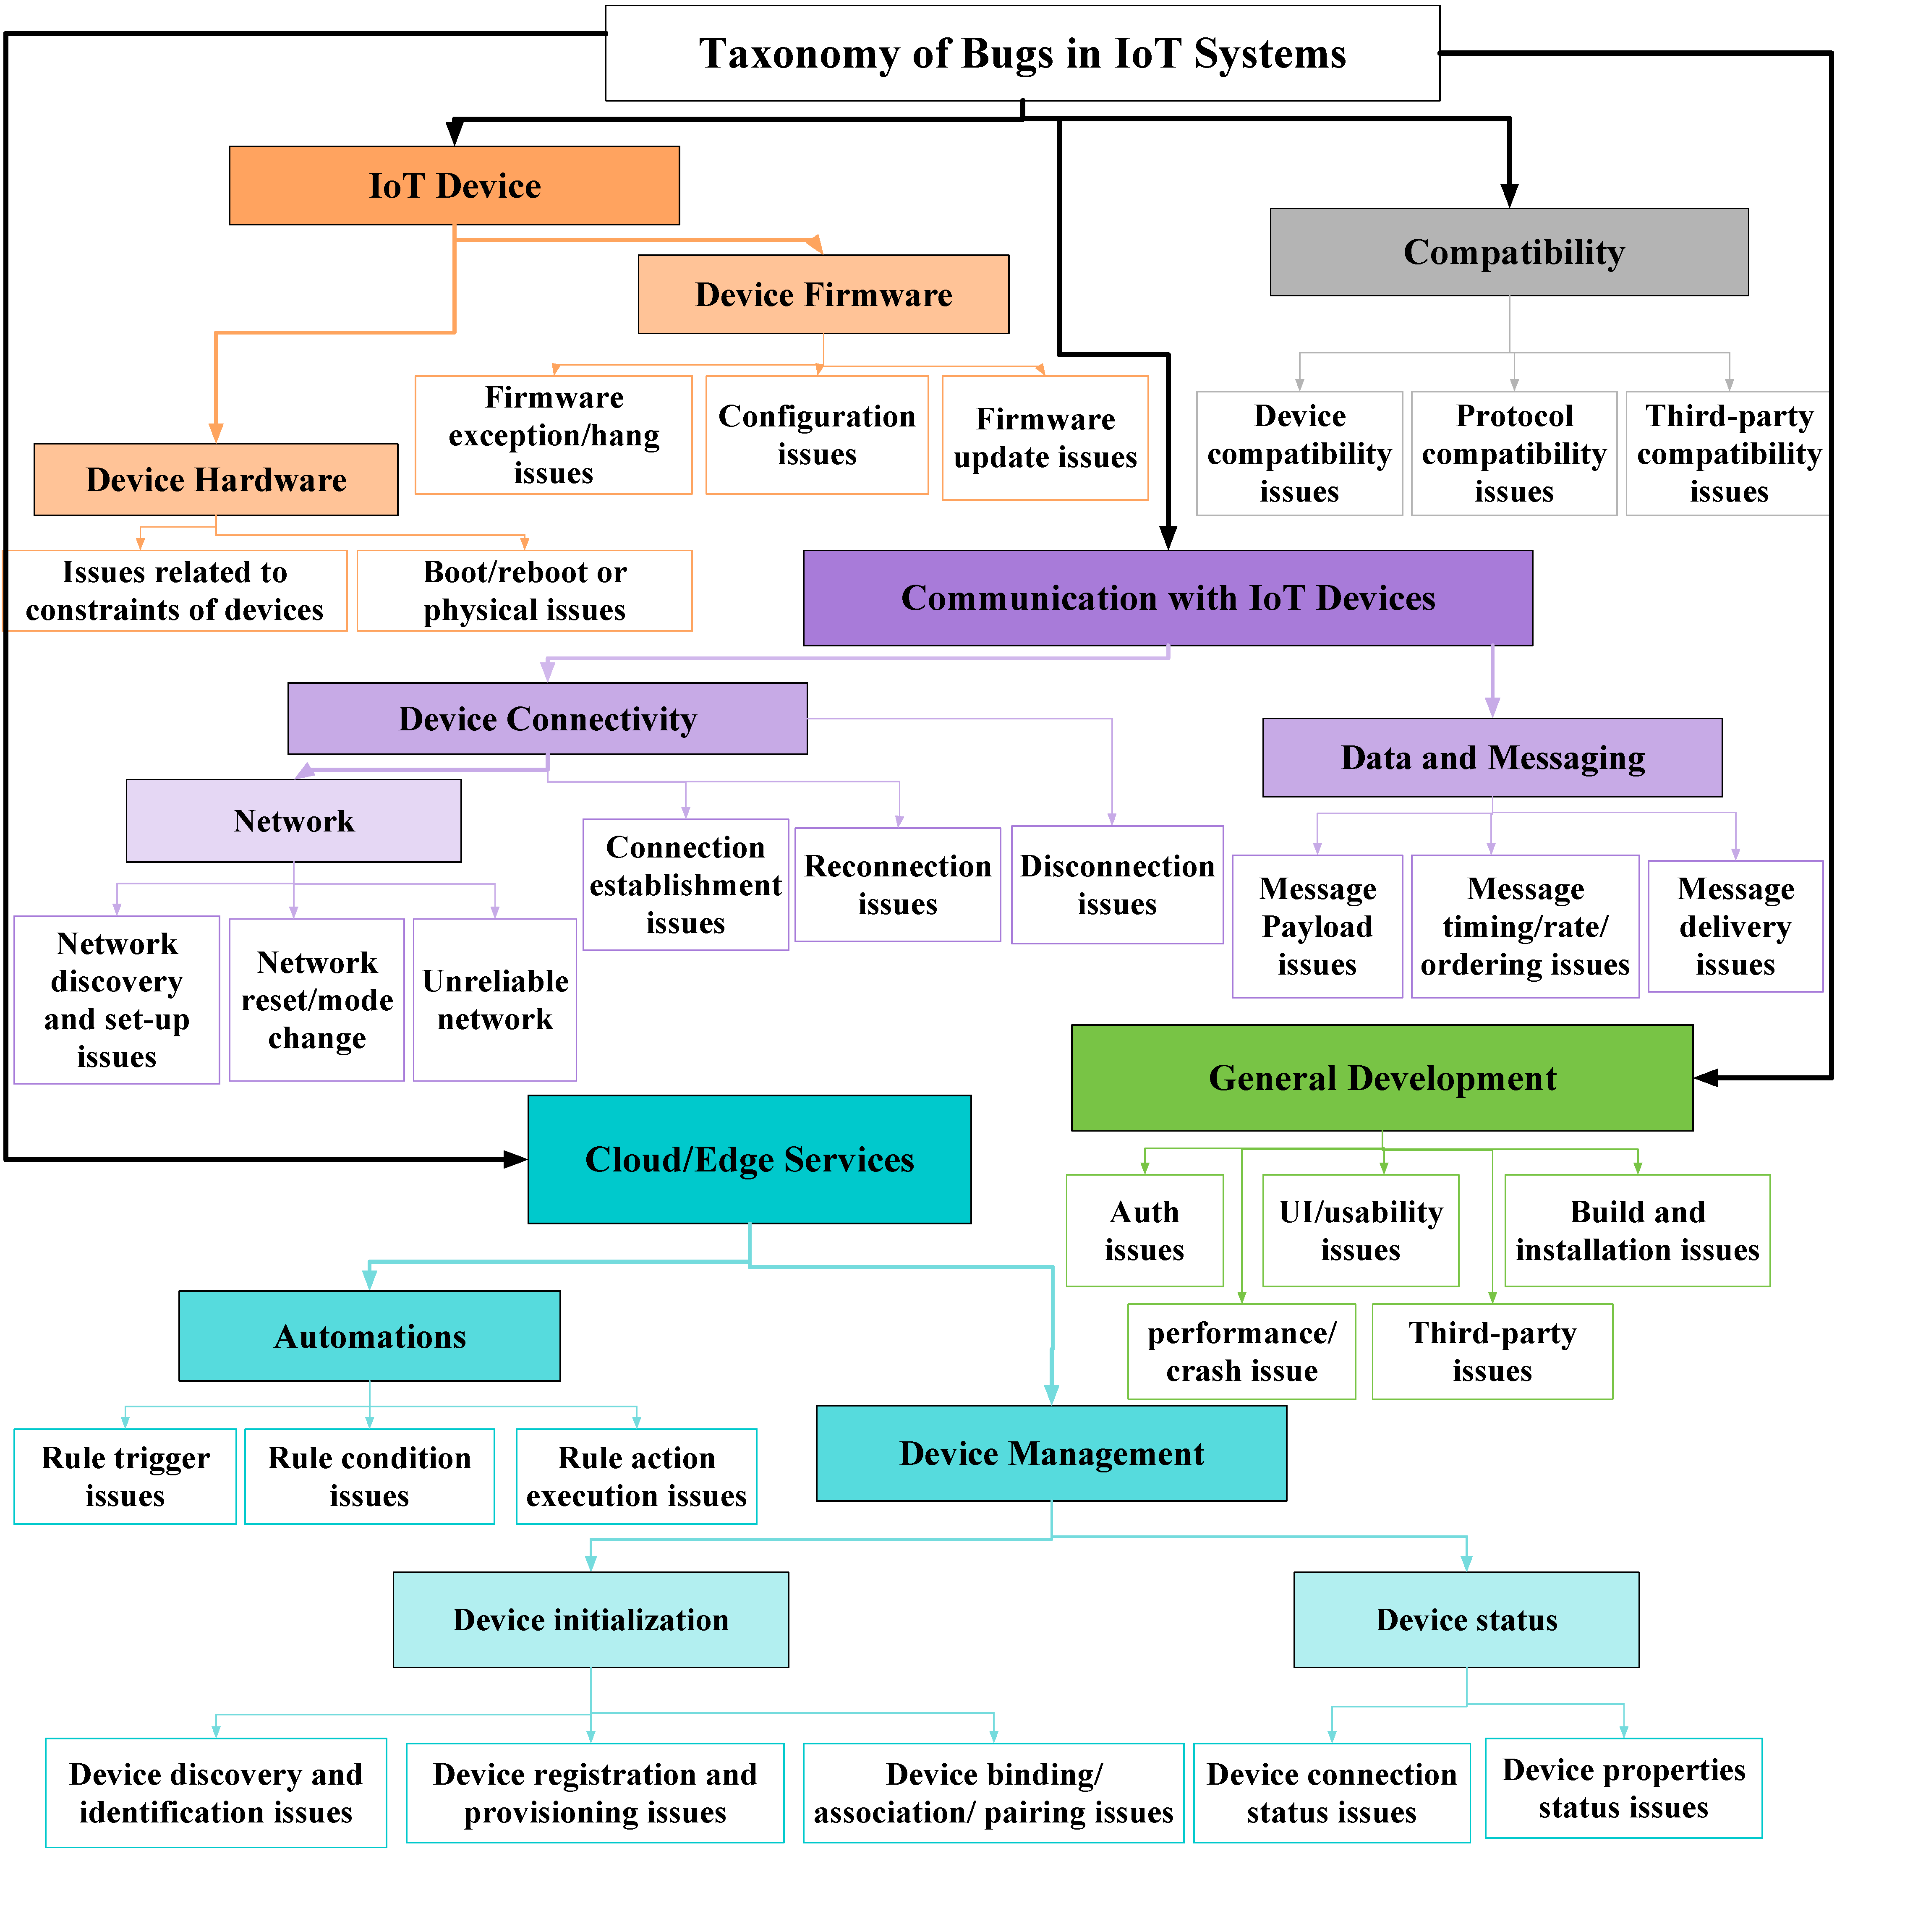
\includegraphics[width=\linewidth]{imgs/tax.pdf}
  \caption{Taxonomy of IoT bugs.} 
  \label{bugTax}
\end{figure*}
\clearpage
}

\textbf{Communication with IoT devices}
Bugs that are related to the communication of IoT devices with each other or with other entities fall under this category. Generally, there are two types of bugs in this category:

\textit{Device Connectivity:} 
Some of the connectivity issues are related to the network that the device relies on for connecting to the internet. One example is when the device cannot discover a valid and available network such as a local access point and therefore loses access to the internet. As it is also mentioned by P\textsubscript{9} \enquote{When the device location is changed to another room or another building, the device has to be reconfigured for the new access point.}

\begin{lstlisting} [language=Java, caption={An example of testing a bug fix after WiFi reconnection in DEVICE-OS/1639}, label={lst:wifiReset}] 
// Initial Wifi Connection
  WiFi.connect();
  // asserting socket creation are done correctly
 const sock_handle_t sock = socket_create();
  if (!socket_handle_valid(sock))   Log.error("socket_create() failed");
 // Asserting that socket connection works without error
 const auto r = socket_connect();
  if (r != 0)  Log.error("socket_connect() failed");
<@\textbf{// WiFi Reconnection and asserting the socket closure operation}@>
 WiFi.off();
 WiFi.connect();
const auto r2 = socket_close(sock);
if (r2 != 0)  Log.error("socket_close() failed");
\end{lstlisting}

 
In addition to the network discovery, not handling a network reset, or unstable and unreliable networks are other common issues that can lead to failures. However, Sometimes IoT devices fail to establish a valid connection to the gateway or remote cloud servers despite a valid network status. Failure in reconnecting, connection refreshing, and ensuring such connectivity failures do not cause propagated failures in other components are other pitfalls that IoT developers often deal with. Additionally, unexpected disconnection or connection closure issues are other manifestations of bugs in this category.

Listing~\autoref{lst:wifiReset} shows a real-world example of the additional tests IoT developers write to check if a fix for a bug caused by WiFi reconnection is a good enough fix. As this example shows, IoT developers have to write code that is able to handle unexpected reconnections and disconnections in order to avoid connectivity bugs.

Additionally, two interviewees (P\textsubscript{6} and P\textsubscript{9}) believe that connectivity bugs are the most serious and challenging bugs. As P\textsubscript{9} states \enquote{the weakest part of our IoT platform is to communicate with IoT devices.}

\textit{Data and Messaging:}
This category includes bugs that are related to data and message sending in the IoT system. Typically, messages are either commands that are sent to IoT devices via the cloud, or they are telemetry data that are received from IoT devices in the edge, cloud, or applications. Some bugs cause failures in delivering these messages from the sender to the receiver. Some other messaging bugs are related to the timing of messages. For instance, various reported bugs are related to the rate and order of the messages. Additionally, some bugs are linked to the payload that is being delivered through the messages. In some cases, payload size or format are the causes of failures. There are also cases where there are violations of payload integrity by messages being truncated or overwritten.


\textbf{Cloud/Edge Services}
This category includes bugs that are related to the services delivered by the remote cloud servers or gateway devices in the edge layer. 

\textit{Device Management:}
To monitor and control each IoT device remotely, devices should be connected to a cloud server or a hub device, and report their status while listening to user commands. Device management (DM) issues include problems that cause failures in this process. 
The first class of DM issues happens in the stage of initializing the IoT device in the cloud or edge systems. One type of device initialization (DI) issue is when the IoT device is not properly or uniquely identified by the cloud or edge components and therefore causes further failures in the subject IoT system. Besides, if the IoT device fails to provide a recognizable identity and valid permissions to the cloud or edge, it would not be allowed to use remote services. Some examples of device registration and provisioning bugs are duplicate device certificates, issues with auto-provisioned devices, or failure in retrieving data from the provisioning service. Another class of DI bugs is problems with binding, association, and pairing of IoT devices. There are several cases where bugs are introduced to the IoT system just because devices are grouped together (such as devices in one room), due to not properly handling the association of a sensor device with a physical object. There is an example mentioned by one of our interviewees (P\textsubscript{5}) where two switches were associated with one lamp and only one switch was working due to issues with addressing multi-instance devices with labels.
The second class of DM issues is related to problems with monitoring the status of IoT devices. One type of device status is the connectivity status, to check whether the device is online, which is also known as the heartbeat check. Some examples of bugs in this type are wrong device heartbeat rate, showing a lost connection as live and vice-versa, or not notifying other components when the device goes offline. Failure in retrieving the device status such as color and brightness for a light bulb, showing the status incorrectly, or failure in updating the device status are some examples of these types of issues.

\textit{Automation:}
This bug category is related to automation services that IoT cloud or edge platforms provide and it is classified into the trigger, condition, and execution issues. Rule trigger defines a condition under which a rule is initiated. Trigger failures usually cause a rule not to become triggered when it should be (SMARTHOME/5578) or vice-versa (HOME-ASSISTANT-CONFIG/2). Rule condition is the statement that should be checked when the rule is triggered. Examples of the rule condition issues are problems in retrieving the device state to check the rule condition since the condition usually relies on device latest status (TESLA-API/43). Issues in the execution of the rule action are the last and the most prominent automation issues. Some examples of these issues are crash after rule action execution, issues in handling asynchronous behavior and threads in rules, and having problems with the output of the rule being unpredictable or nondeterministic.

\textbf{General Development}
This category captures common development bugs. Some common issues are problems with installing, compiling, or building a project as well as unexpected crashes or performance issues in the IoT project. The general development category also includes bugs in the authentication or authorization process. One of the IoT-specific authorization issues are problems with generating, signing, or maintaining the certificates that devices have to present for using cloud or edge services (AZURE-IOT-SDK-C/657). Other sub-categories of general development bugs are UI-related, usability, or external issues.

\subsection{Root causes of Bugs}

\afterpage{%
 \begin{figure*}
  \centering
   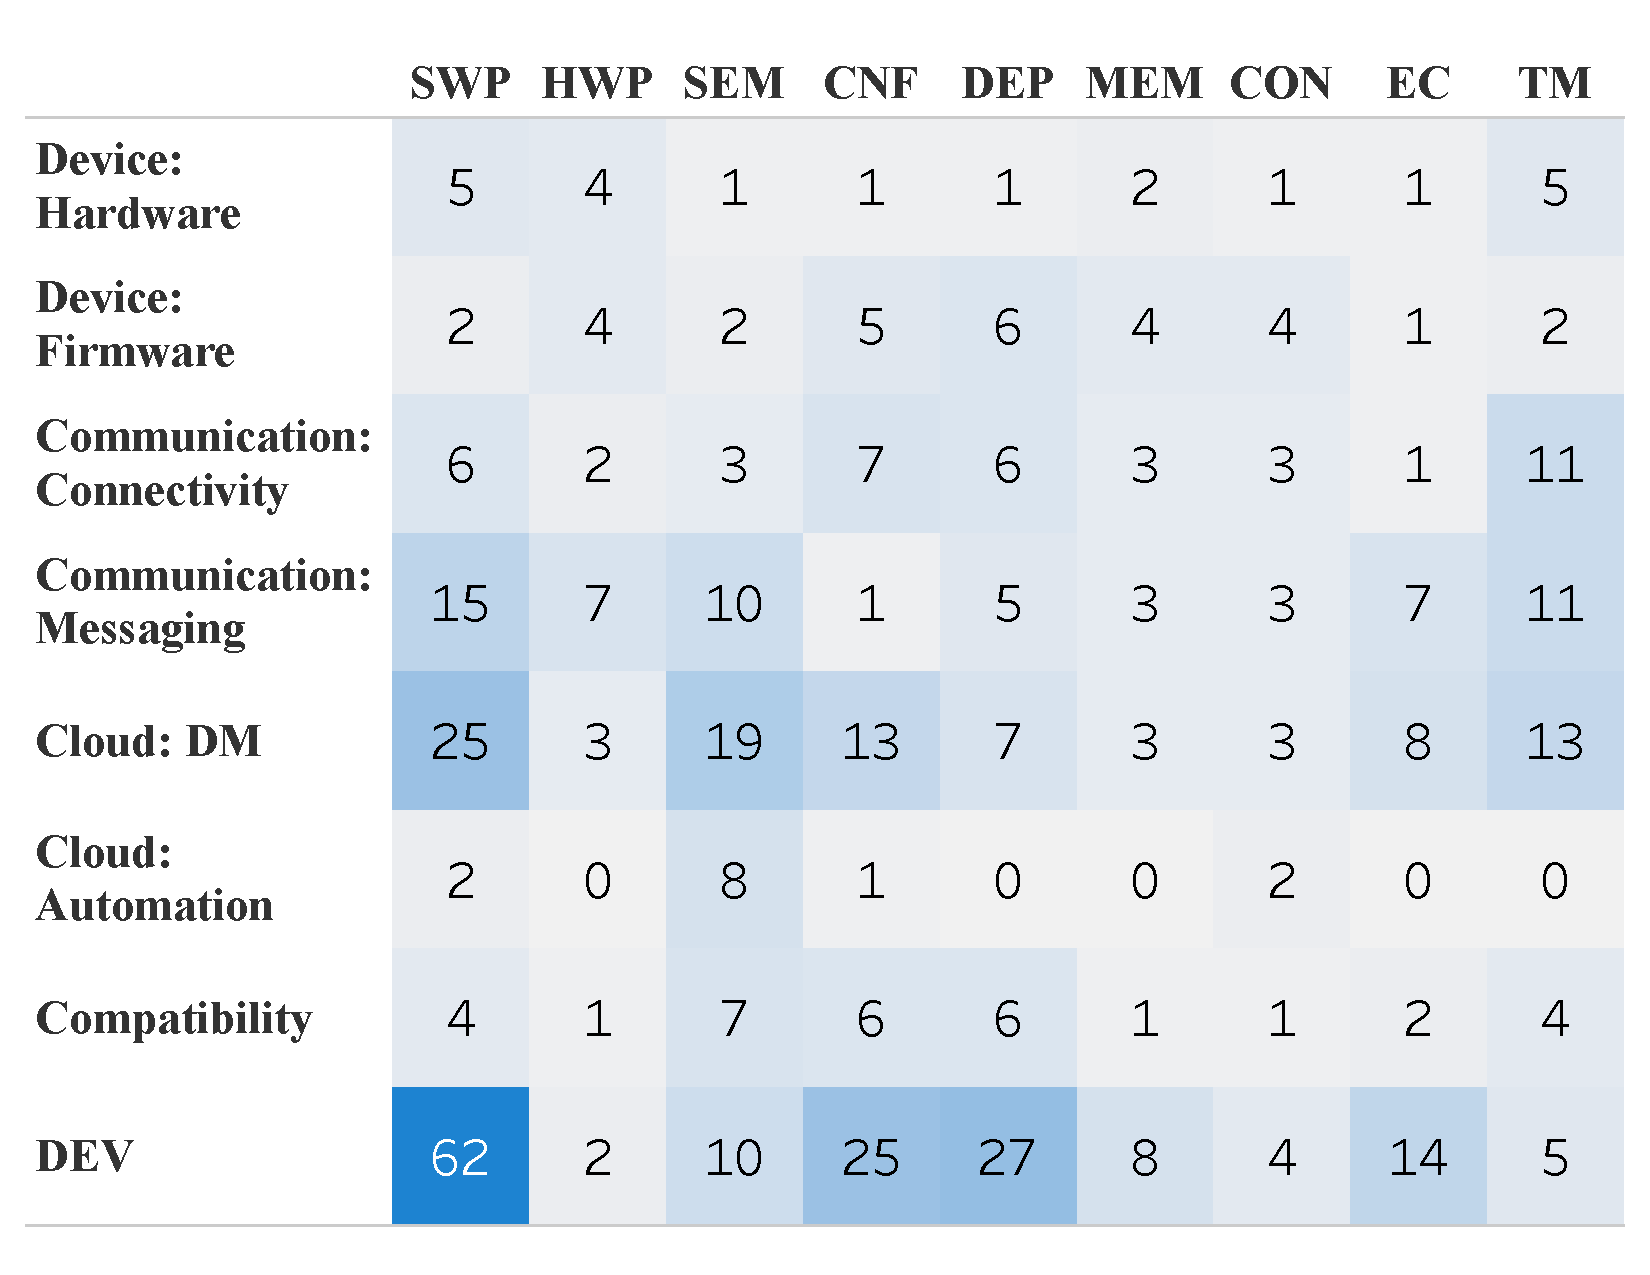
\includegraphics[width=\linewidth]{imgs/rcvis.pdf}
  \caption{Distribution of bug categories (vertical) and root causes (horizontal)}
  \label{fig:bugRC2d}
\end{figure*}
\clearpage
}

Figure \ref{fig:bugRC2d} shows the distribution of bug categories and root causes. In this section we will describe each category of root causes. 

\textbf{General software programming faults (SWP)}: These faults are the most dominant root causes of the bugs. These faults are often syntactical mistakes by IoT developers. Examples of such faults would be accessing null pointers or empty memory locations, typos, missing/wrong conditions/loops, or missing/wrong values in code, infinite loop, and wrong data type. Also, we consider all UI-related faults to be in this category, like faults in the front-end code of a web application or an Android or iOS application. The top three issues caused by these faults are messaging issues, device management issues, and general development issues.


\textbf{Semantic programming faults (SEM)}: These faults are the second most dominant root causes of IoT bugs. After general development issues, top issues caused by SEM faults are device management issues, automation issues, and compatibility issues. Some semantic mistakes that IoT developers make are wrong control flow, faulty logic of functionalities, or erroneous return values. 

One example of faulty return values is the mistake in AZURE-IOT-SDK-C/481, when the developer wants to get a device with a certain ID. If the device ID does not exist, the expected behaviour is to create a new device with that ID and return the newly created device. However, if a device with a certain ID does not exist, the IoT platform mistakenly returns an error code which is a fault in the return value.

Some SEM faults are related to the automation logic of the IoT system, such as logical faults in automation apps, which are also discussed in recent studies~\cite{ISSTA2020Interactions}.  An example of such mistakes is obvious in ENTITY-CONTROLLER/103, where developers have conflicting opinions on the expected behaviour of IoT devices when an overriding command is sent to devices. This issue gets more serious when the expected behaviour designed by developers as the correct behaviour, does not support certain user scenarios, which is the case in this bug example.

\textbf{Dependency faults (DEP)}: The next frequent root cause is DEP faults, where developers use wrong versions of the software or firmware libraries, tools, devices, or protocols. Dependency faults are the main causes of compatibility issues, device firmware issues, and general development issues. It's important to note that dependency faults are different from compatibility bugs in nature since the latter is mostly an observed failure that can have different causes (as we can see in \ref{fig:bugRC2d}), where the first one is a fault by developers in choosing the right version. Developers have to follow the dependency constraints among hardware devices and software libraries to avoid these faults in their code.

\textbf{Timing faults (TM)}: One of the most important root causes often leading to hardware, connectivity, and messaging issues are TM faults. Improper handling of time-outs or rate of operations, wrong time-out values for connection closures, or not handling asynchronous behaviors are among timing-related root causes. In some cases, the connection is monitored to be closed when the device is idle. Furthermore, finding the ideal time-out value for properly closing the connection to avoid possible failures has shown to be a faulty task for IoT developers.

One example of TM faults occurs in DEVICEHIVE-JAVA-SERVER/145 when users want to get a specific command of a certain device and instantly receive an empty array as the response when the device is still busy executing the same command from before. The expected behaviour is to wait until the device acknowledge the complete command execution within the defined time-out. Figure~\autoref{fig:tm} shows part of the bug fix for this issue, that enforces the device to first wait for the command to be processed.

 \begin{figure}[ht]
  \centering
   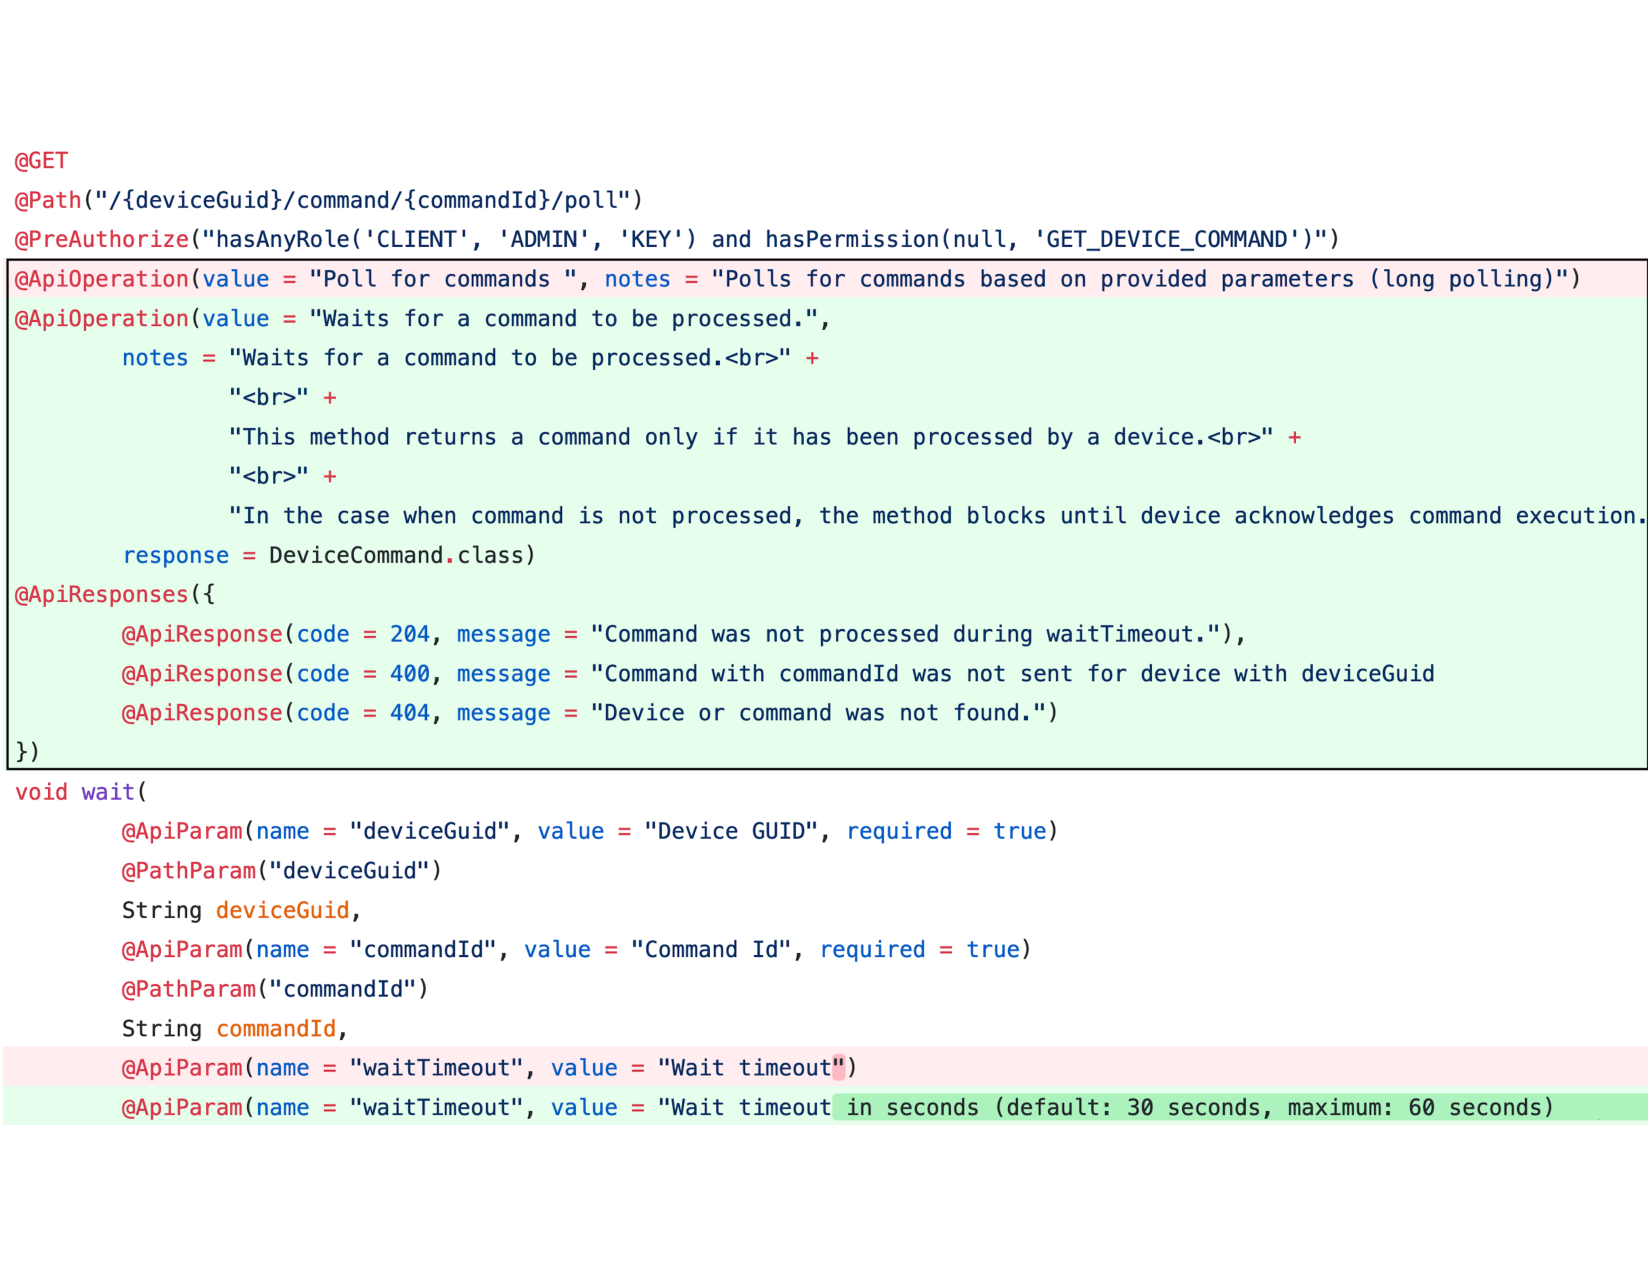
\includegraphics[width=\linewidth]{imgs/TM}
  \caption{A timing fault while polling device commands occurred in DEVICEHIVE-JAVA-SERVER/145}
  \label{fig:tm}
\end{figure}


\textbf{Hardware programming faults (HWP)}: Some faults that are more specific to hardware programming such as interrupt handling, are assigned to the category of HWP faults. Examples include wrong pin/port mapping, improper socket operation, wrong bit assignment, and incorrect interrupt handling. Other faults in hardware code resemble those in software code, like referencing a null pointer or wrong return type.

\textbf{Faults in handling exceptional cases (EC)}: These faults are another root cause for IoT bugs that include mistakes in handling corner cases (large or out of range data), not handling errors properly, or not handling changes of the requirements or changes in third-party components. Figure~\autoref{fig:rc8} shows a EC fault in which the IoT developers did not count for large messages.
 
 \begin{figure}%[h]
  \centering
   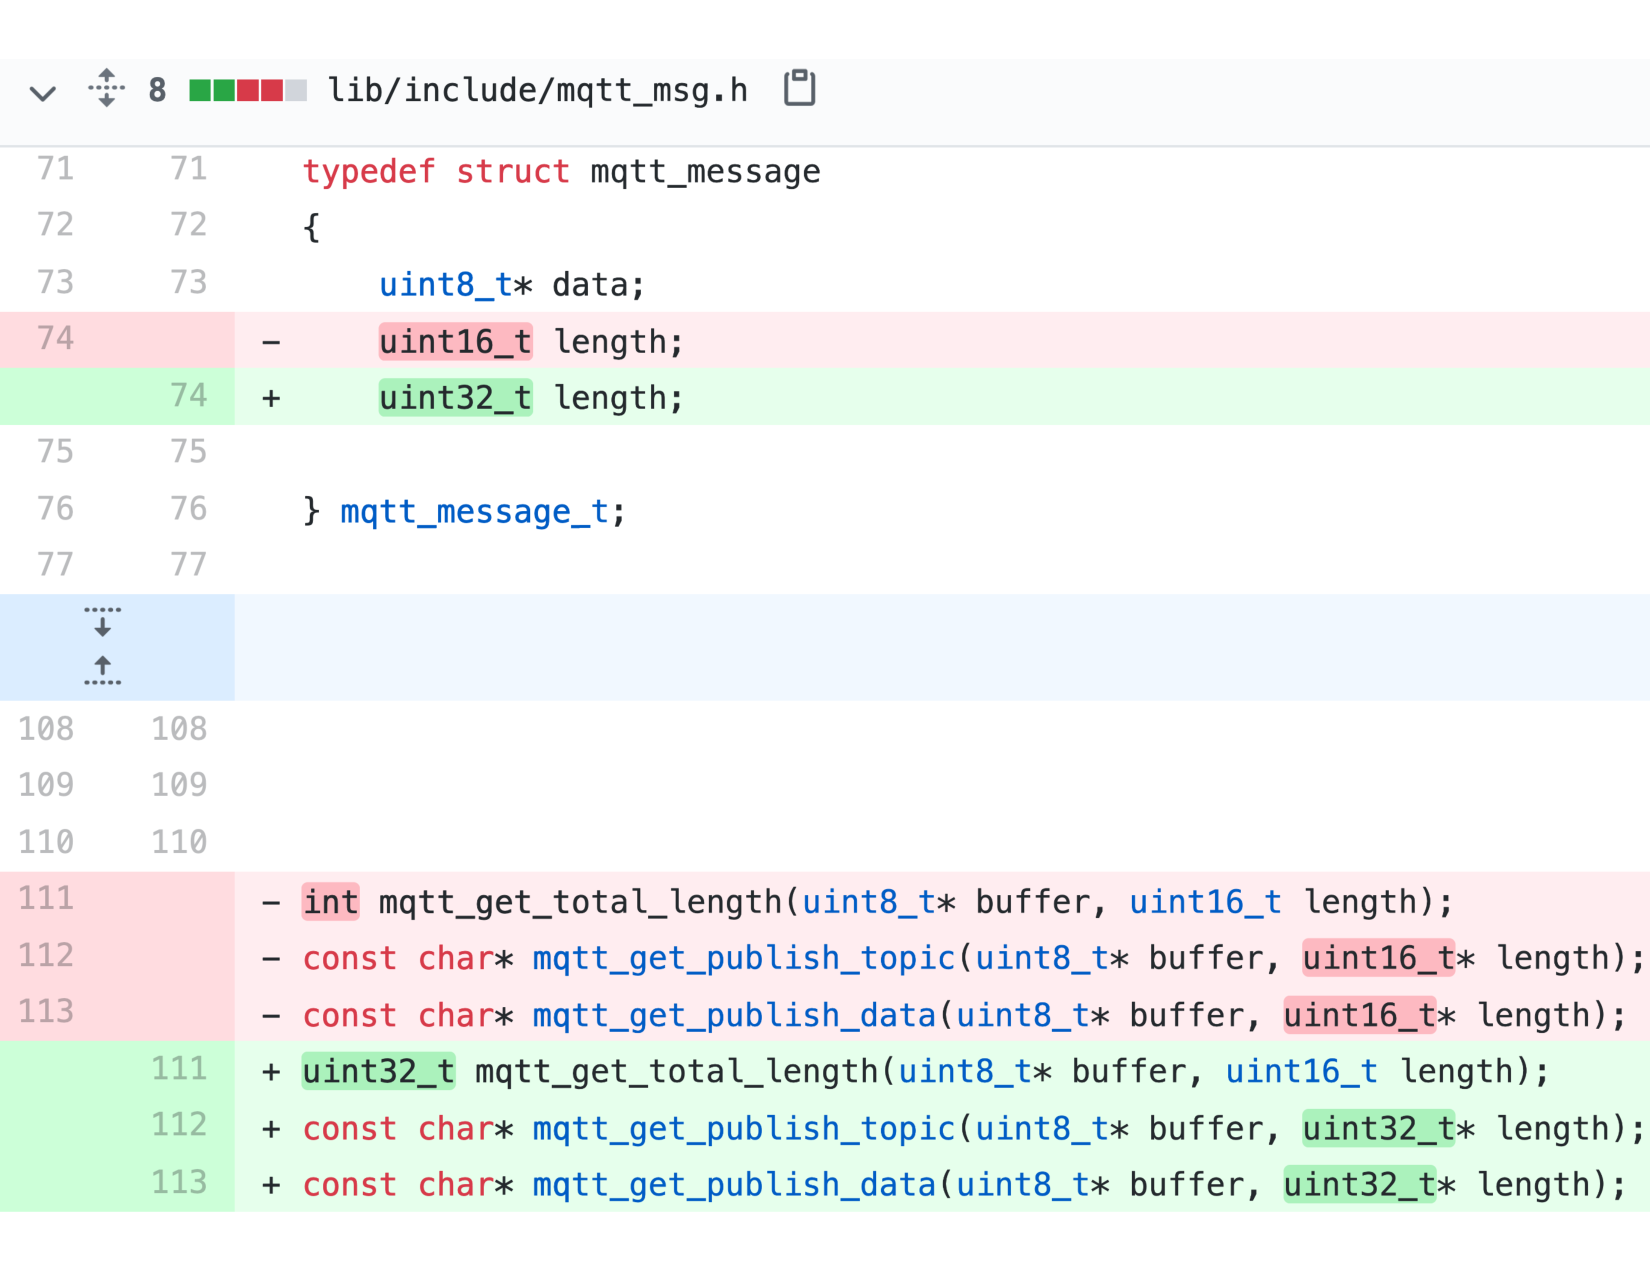
\includegraphics[width=\linewidth]{imgs/rc8}
  \caption{An EC fault (from ESP-MQTT/34) that allocates 16 bit instead of 32 bit for each MQTT message, which cause the system to break with large MQTT messages.}
  \label{fig:rc8}
\end{figure}
 
\textbf{Memory faults (MEM)}: Faults related to incorrectly handling memory objects fall into this category. There are some previous studies focused specifically on memory-related bugs \cite{memBugs}. Also some other studies have categorized these bugs as a defect in software systems \cite{openSourceBugs}. Memory bugs often happen as the result of race conditions on memory locations. A race condition is a situation in which the result of an operation depends on the interleaving of certain individual operations. Such situations can lead to different types of bugs like buffer overflow, stack smashing, memory leak, uninitialized read, and double free bugs, as it is also classified in bugBench \cite{bugBench}.

\textbf{Concurrency faults (CON)}: A concurrency fault exists if running two threads at the same time is not handled properly. These faults usually do not show up if the two programs run sequentially. Thus, these bugs happen only in multi-threading or multi-processes environments and only when the operations are ill-synchronized. In the context of IoT, the communication of things and the cloud can be asynchronous, which means data can be transmitted intermittently rather than in a steady stream, because there are various parties (user, sensor, actuator) that can send data whenever they like. Based on the classification in bugBench, there are three types of concurrency bugs. Data race bugs happen when at least two threads access a shared variable at the same time. At least one thread tries to modify the variable. Atomicity-related bugs happen when one thread is unexpectedly interrupted by another thread. Deadlock is a situation when two or more threads wait for a resource and can never proceed anymore. 


\textbf{Configuration faults (CNF)}: Hardware devices and development tools need some particular configuration, and wrong provisioning of the proper configurations are considered CNF faults.


\subsection{Correlations among bug categories}
During our analysis, we observed some frequent patterns of certain bug categories appearing together more often. To study the correlations between bug categories, we used Lift~\cite{kamber2001data}, a statistical metric introduced by Han and Kamber that computes the probability of two categories appearing together. For each pair of bug category, a lift value of more than 1 shows a positive correlation, and a lift value below 1 reveals a negative correlation. 

Table \ref{tab:correlations} shows the lift values of correlated bug category pairs. The top correlated bug categories are [hardware, firmware], [hardware, connectivity], and [firmware, connectivity]. This correlation analysis, besides helping IoT developers in debugging, gives insight into how intertwined IoT bugs can be in practice.


 \begin{figure}%[h]
  \centering
   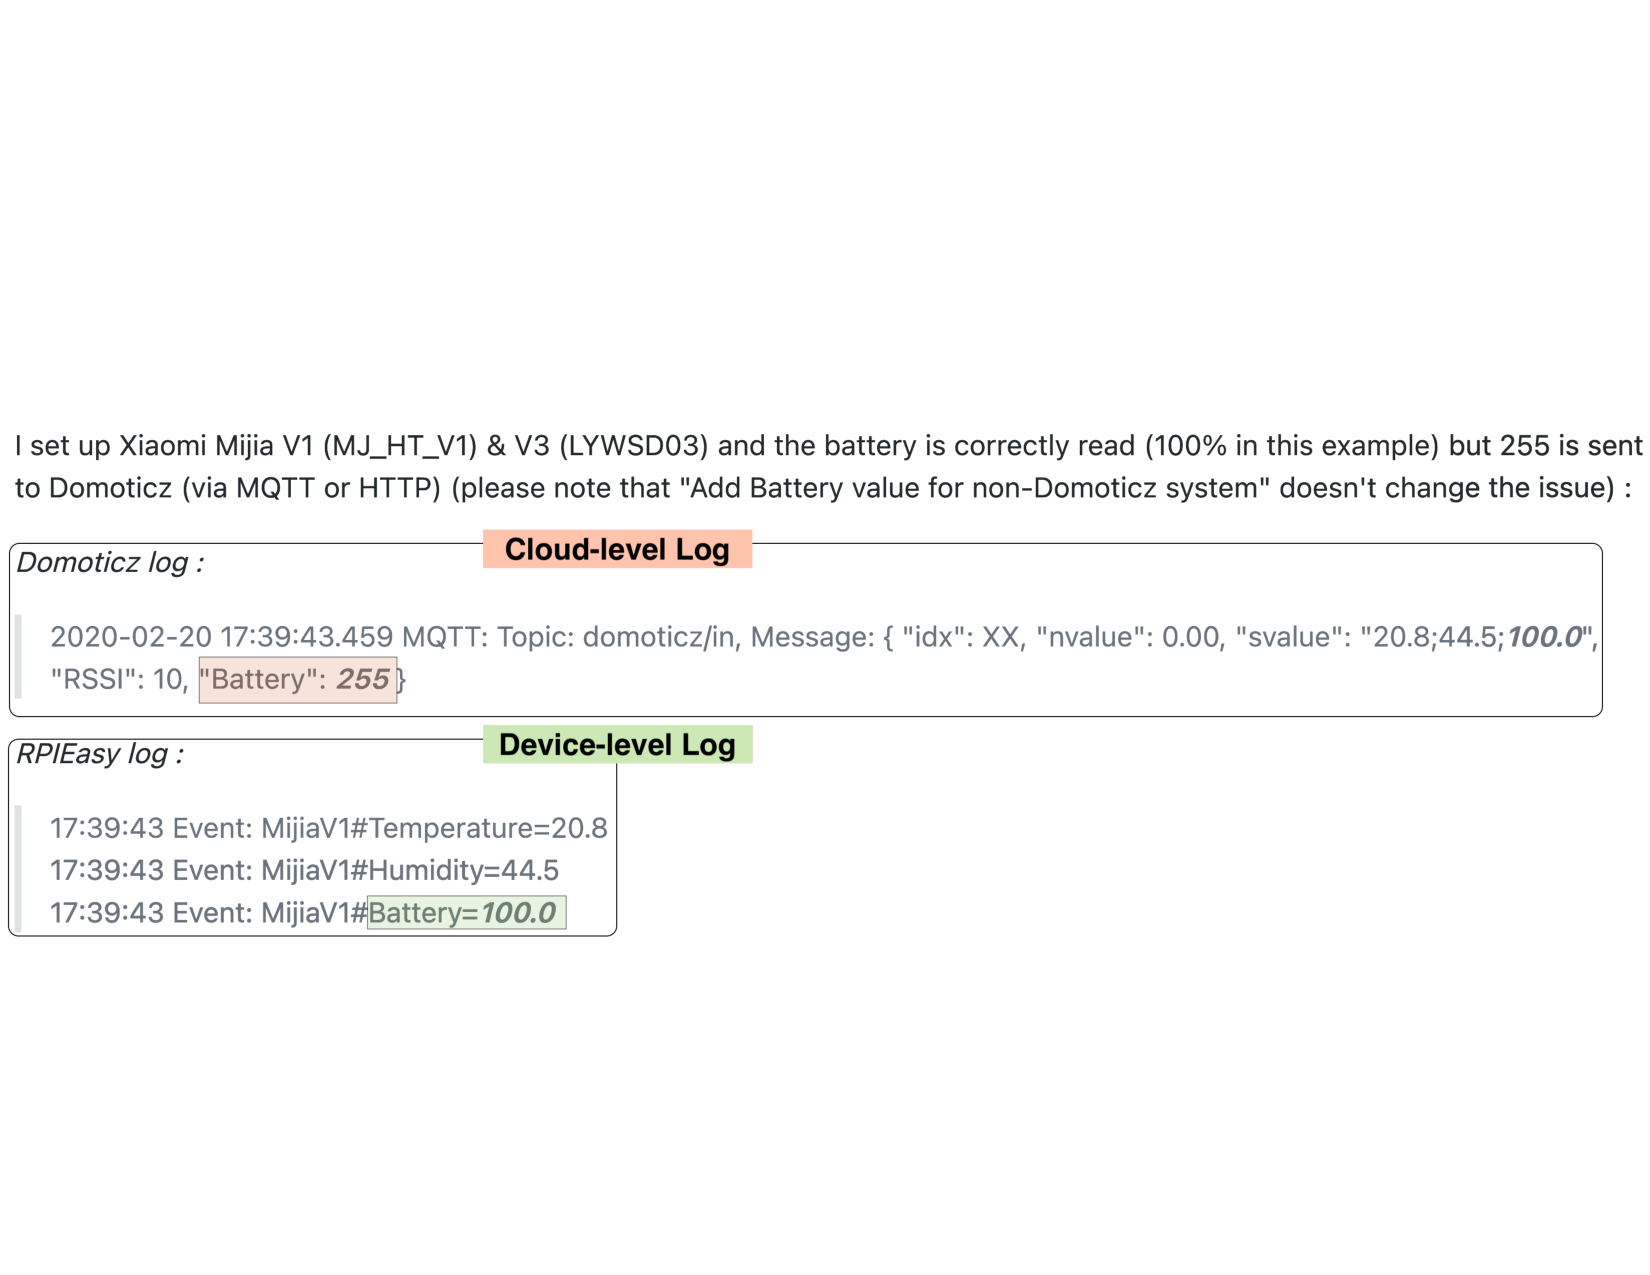
\includegraphics[width=\linewidth]{imgs/corEx}
  \caption{An example of how a fault in the device layer has propagated to a failure in the cloud layer}
  \label{fig:corEx}
\end{figure}


As the Figure~\autoref{fig:corEx} shows the GitHub discussions for RPIEASY/128, an IoT developer observed a clear conflict between the device status logged from the device layer and the cloud layer. Further investigation revealed that a fault in the device driver code has caused the wrong device battery status to be sent to the IoT cloud.

 \begin{table}[htbp]
\caption{Bug Categories with Positive Correlation}
\begin{center}
\resizebox{\linewidth}{!}{%
\begin{tabular}{l l | r}
\hline
\textbf{Bug Category}& \textbf{Bug Category }& \textbf{Lift Value}  \\
\hline
Device: Hardware& Device: Firmware& 3.86   \\
Device: Hardware &Communication: Connectivity & 2.57   \\
Device: Firmware &  Communication: Connectivity & 2.25   \\
Compatibility &  Cloud: Device Management & 1.84   \\
Compatibility &  Communication: Messaging & 1.44   \\
Communication: Messaging & Device: Firmware  & 1.42   \\
Cloud: Device Management & Automation  & 1.38   \\
Cloud: Device Management & Device: Hardware  & 1.28   \\
Communication: Connectivity&Communication: Messaging & 1.22   \\
Communication: Connectivity& Compatibility & 1.14   \\

\hline
\end{tabular} }
\label{tab:correlations}
\end{center}
\end{table}


\subsection{Frequency and severity of bugs}

The most frequent categories of bugs are general development issues (48\%), device management issues (29\%), and messaging issues (19\%). 

We asked our survey participants whether and how frequently they face each bug (sub)category and what are their perceived severity based on the impact on the IoT system and fixing-time. Table \ref{tab2} shows the results.  All the bug categories in our taxonomy have been faced by at least 82\% of IoT developers, which shows the bug categories are representative of the real-world bugs in IoT systems. Connectivity issues are the most frequent and severe bug category with more than 97\% of IoT developers have faced it at least once. more than half of developers face it frequently, and 62\% of IoT developers find it severe. After this category, messaging, automation, and device management issues are among the most approved bug categories with all of them approved by more than 90\% of IoT developers. 

In terms of frequency, hardware, and messaging issues are among the most frequent bug categories after connectivity issues. 

Device-related issues are the least experienced bug categories, but they are the most severe bugs after connectivity issues. According to the survey respondents, automation issues are the least severe bugs, however, more than 91\% of IoT developers have faced them at least once. The compatibility issues are the least frequent bugs according to IoT developers' experiences.

Regarding sub-categories, device initialization issues are the most frequent and severe device management bugs since about 95\% of IoT developers having dealt with them, and more than half of developers find it severe. 

Also concerning the device status issues, bugs related to the status of connection have shown more frequency while bugs related to the status of device properties are more severe based on survey respondents. Among device-related issues, bugs that are related to the constraints of IoT devices have the most frequency. The device firmware exception issues are the most severe device-related bugs. Concerning general development issues, installation issues are the most frequent and severe bugs. 

Bugs related to authentication and installation are the least experienced general development bugs. Nevertheless, more than 81\% of IoT developers have the experience of dealing with them and nearly 30\% of survey respondents find this bug severe.


 \begin{table}%[htbp]
\caption{Survey Results: Bug Taxonomy}
\resizebox{\linewidth}{!}{%
\begin{tabular}{ l | r | r r r | r }
\hline
\multicolumn{1}{l|}{\textbf{Bug Category}} &\multicolumn{1}{l|}{\textbf{Have faced}}& \multicolumn{3}{c|}{\textbf{Frequency}}& \multicolumn{1}{c}{\textbf{Is Severe}} \\
& &Frequently&Sometimes& Rarely&  \\
\hline
Device: Hardware&82.50\% &30.30\% &39.06\% &30.64\% &43.61\%  \\
Device: Firmware&85.75\% & 24.20\%& 44.48\%& 31.32\%& 42.78\% \\
Communication: Connectivity& 97.22\% &50.29\% &38.29\% &11.42\% &62.78\% \\
Communication: Messaging&92.22\% &33.74\% &36.14\% &30.12\% &40.56\% \\
Cloud: Device Management& 90.93\% &25.06\% &46.43\% & 28.51\%&40.75\% \\
Cloud: Automation& 91.67\%& 20.00\% &44.24\% &35.76\% &32.22\% \\
Compatibility& 86.11\% &23.88\% &40.00\% &36.12\% &36.11\% \\
Dev&87.89\% &24.53\% & 39.44\%&36.03\% &38.89\% \\
\hline
\end{tabular} }
\label{tab2}
\end{table}

\textbf{Taxonomy augmentation}
Regarding IoT bugs, we collected 79 tags from interviews and 18 tags from the survey comments. Device binding issues, performance issues, and third-party compatibility issues were not discovered before the interviews and were added by interviewers' experience. The survey comments did not reveal any new information to be added to the taxonomy. However, the extracted tags, from both the interviews and survey, helped us to characterize each bug category by providing contextual data.


\subsection{Threats to Validity}
\textbf{Internal validity}
One internal threat to the validity of our study, similar to most qualitative studies, is researchers' bias in coding qualitative data. We mitigated this risk by having all authors of the paper involved in the tagging process and discuss any discrepancies in tags for all pieces of qualitative data from various sources (bug reports, interview transcripts, survey comments). For interviews specifically, we eliminated any personal preference on our results by triangulation; each piece of meaningful data from interview transcripts was tagged by one researcher who conducted the interview and one who was not present in the interview session.

\textbf{External validity}
One external threat to the validity of our study is the generalization of studied IoT repositories. We minimized this issue by studying a large number of repositories (91 repositories) selected from all layers of IoT systems. Another risk to the validation of our study is the interview and survey participants not being representative of all IoT developers. However, we minimized this risk by recruiting interview and survey participants with different IoT-related field of expertise, years of experience, companies, and domains. In addition, our survey is filled out by 194 IoT developers with a diverse distribution of skills and experiences.

All our study material, including the bug dataset and interview and survey questions, is available online~\cite{repPack}.

\endinput


%%% The following is a directive for TeXShop to indicate the main file
%%!TEX root = diss.tex

\chapter{Challenges}
\label{ch:Challenges}

\section{Methodology}


\section{Findings}
In this section, we provide our findings regarding the challenges faced by IoT developers.

\subsection{Testing and Debugging Challenges}
\textbf{Relying on access to the real device}
According to seven interviewees, several GitHub issues (DEVICE-OS/1871, MYCONTROLLER/485, TESLA-API/43), and 74\% of survey participants, IoT developers rely on access to devices to test and debug their IoT system, by tasks such as manual reset or device output monitoring (P\textsubscript{2,3,7}).


In some scenarios, devices are out of reach or in hard-to-access locations thus making remote debugging more essential. 
Four interviewees believed that practical simulation solutions are required for better IoT testing and debugging. As P\textsubscript{5}, a middleware developer stated \enquote{IoT device vendors do not provide a mock of their devices, and we have to do reverse engineering on the actual hardware devices rather than working with the simulated ones.} Also as P\textsubscript{5,8,9} stated, current simulation solutions in IoT are not mature enough and they are only valid for limited scenarios, such as testing high-level controllers or small unit tests, rather than being suitable for all levels of testing such as system testing.

 \begin{table}%[htbp]
\caption{Survey Results: Bug Taxonomy}
\resizebox{\linewidth}{!}{%
\begin{tabular}{ l | r | r r r | r }
\hline
\multicolumn{1}{l|}{\textbf{Bug Category}} &\multicolumn{1}{l|}{\textbf{Have faced}}& \multicolumn{3}{c|}{\textbf{Frequency}}& \multicolumn{1}{c}{\textbf{Is Severe}} \\
& &Frequently&Sometimes& Rarely&  \\
\hline
Device: Hardware&82.50\% &30.30\% &39.06\% &30.64\% &43.61\%  \\
Device: Firmware&85.75\% & 24.20\%& 44.48\%& 31.32\%& 42.78\% \\
Communication: Connectivity& 97.22\% &50.29\% &38.29\% &11.42\% &62.78\% \\
Communication: Messaging&92.22\% &33.74\% &36.14\% &30.12\% &40.56\% \\
Cloud: Device Management& 90.93\% &25.06\% &46.43\% & 28.51\%&40.75\% \\
Cloud: Automation& 91.67\%& 20.00\% &44.24\% &35.76\% &32.22\% \\
Compatibility& 86.11\% &23.88\% &40.00\% &36.12\% &36.11\% \\
Dev&87.89\% &24.53\% & 39.44\%&36.03\% &38.89\% \\
\hline
\end{tabular} }
\label{tab2}
\end{table}

Some relevant challenges mentioned in the survey are \emph{affording to have all types of IoT devices}, \emph{complex custom logic for effective IoT device mocking and simulation}, and \emph{setting up test environments with IoT devices}. 

\textbf{Fault localization}
According to eight interviewees, nine survey comments, and also half of the survey participants, fault localization is a barrier due to lack of transparency in the operations of IoT systems. As P\textsubscript{7} mentioned \enquote{there is no environment that logs everything.} One contributing factor to this is the difficulty of tracing executions of numerous external components in IoT systems. P\textsubscript{3} mentioned using open-source solutions just to be able to log everything. 


Another factor that impacts fault localization is the existence of hidden failures. 

As an example, P\textsubscript{7} mentioned \enquote{It's hard to recognize on the app that the temperature the device is reporting now is for several minutes ago.} Besides, P\textsubscript{2,4} mentioned examples of failures that only show up after the device has worked for a specific amount of time (five minutes for P\textsubscript{2}, several hours for P\textsubscript{4}), which is also observed in GitHub issues (DEVICE-OS/1926, ZWAVE2MQTT/141, VSCP/207). This issue makes IoT failures more unpredictable and may hide developers' faults. Another issue toward fault localization is the lack of tools and developers' support. For instance, P\textsubscript{3} inspects device messages in bit-level by monitoring communications using Wireshark. P\textsubscript{2}, as a hardware platform developer, said \enquote{Since there is no feedback of errors or corruptions from devices, we've added some LEDs to them to track if something is working in the device level or not.}


\textbf{Reproducing IoT bugs}
In addition to observing several GitHub discussions (DITTO/414, TESLA-API/68), we collected four tags from interviews, and three survey comments regarding the challenge of reproducing IoT bugs. Besides the already mentioned factors which harden bug reproduction, such as limited access to devices or hidden failures, some bugs only happen with a specific device setting or with certain environments of the IoT system. IoT developers cannot reproduce these bugs unless they have exactly the same setting or environment. For instance, a survey comment indicated \enquote{It's hard to reproduce some memory-related bugs in X86 devices when they have ASLR enabled.}
% due to existence of ASLR mechanism in these devices that interfere with these bugs
Also, we observed other examples such as TEMPERATURE-MACHINE/13: \enquote{I can reproduce the bug with the help of ice packs taken at three different temperatures from my freezer.}

\textbf{Combinatorial explosion}
In addition to all the evolving components in traditional software, such as libraries and operating systems, there are more changing factors in IoT systems. Hardware devices produced by various manufacturers with different standards, device integration middlewares, and communication protocols are some examples of these extra changing factors in IoT. With all these components releasing new versions at a specific rate, a combinatorial explosion problem is likely to happen when developers want to cover all possible combinations with test cases.
One relevant statement is \enquote{I do not have all kinds of bulbs, remotes, and sensors, so I could be completely wrong!} in a GitHub discussion (PYTRADFRI/135). We could collect eight tags come from four interviewees and two tags from survey comments regarding the challenge of combinatorial testing. As one example, P\textsubscript{9} said \enquote{We have to test with 10 or 15 different devices each time}. Also, 80 percent of survey respondents agree with the combinatorial explosion as a testing challenge for IoT developers, and P\textsubscript{8} mentioned it as the most severe testing challenge. 

\textbf{Testing and debugging edge-cases}
Covering large-scale scenarios (e.g. too many devices) and exceptional cases (e.g. temperatures below zero) add to the test coverage obstacles. This challenge is mentioned by four interviewees, three survey participants, and observed in several GitHub discussions (DEVICE-OS/1926, TEMPERATURE-MACHINE/13). As one example, P\textsubscript{4} said \enquote{We should put effort to write proper tests against concurrency issues since we should be able to handle 140,000 HTTP requests per second because our IoT system is deployed in different cities.} Additionally, this challenge is the most experienced testing challenge (83\% of respondents). 

\textbf{Immature testing culture}
Figure~\ref{fig:testing} shows an over-reliant on IoT developers for testing as 64\% of participants mentioned developers are the main testers in their IoT project.


As P\textsubscript{6}, a developer of a popular IoT project with near 7K stars, stated \enquote{We do not have a QA team. it's up to developers to do testing, either manually or writing automated tests.} Often, software developers do not have the skills to test the hardware side. P\textsubscript{9}, a software developer of an IoT platform with 1.5K stars, told that the bottle-neck of their IoT platform is testing the hardware side since they do not have sufficient knowledge for tools and practices of hardware testing.


As Figure~\ref{fig:testing} shows, IoT testing highly depends on manual tasks as only 5\% of participants reported testing completely automatic. Also, during interviews, four interviewees mentioned manual approaches for IoT testing. According to the survey respondents, the most adopted IoT testing approach is hybrid strategies. An example of such an approach is described by one IoT developer \enquote{Services which don't interact with devices directly are tested automatically, but checking the entire platform with devices requires manual testing.} 


 \begin{figure}%[h]
  \centering
   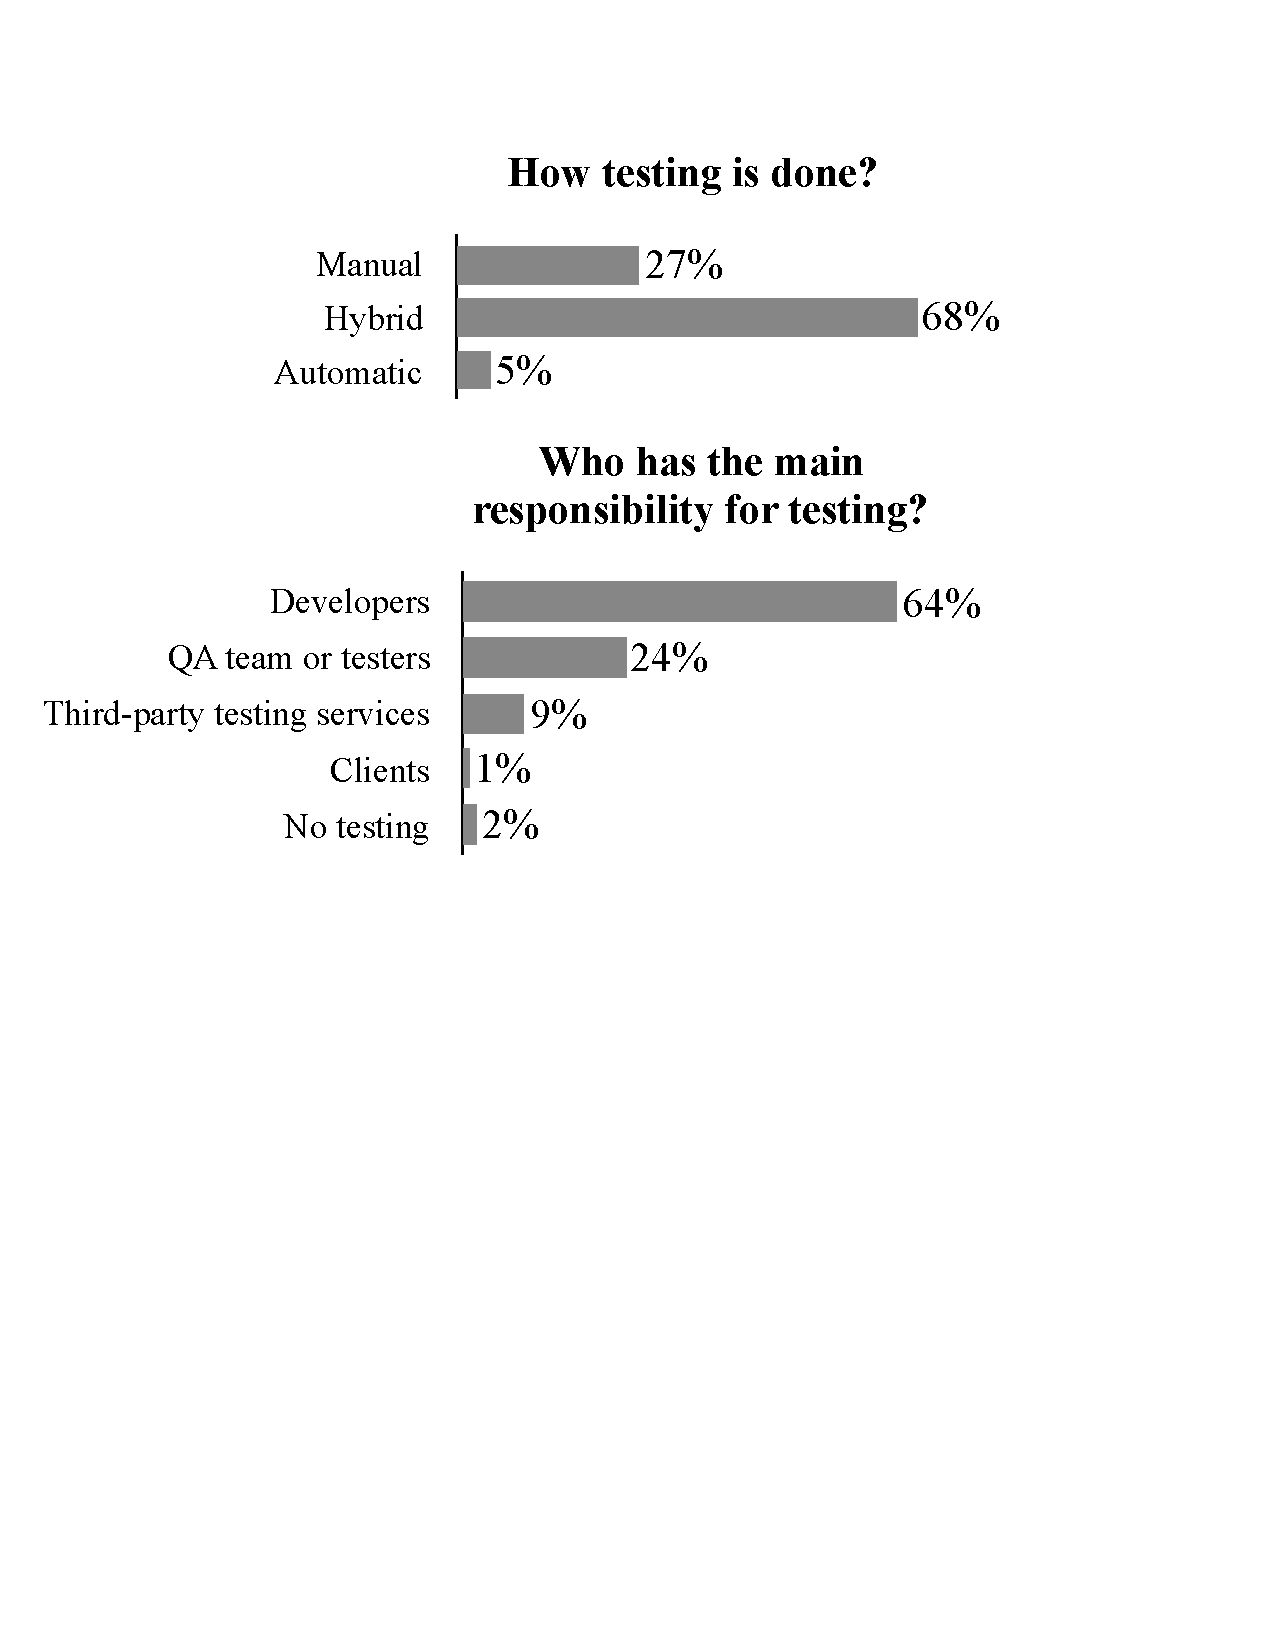
\includegraphics[width=\linewidth]{imgs/testing.pdf}
  \caption{Survey responses about testing in IoT projects.
  }
  \label{fig:testing}
\end{figure}

\subsection{Heterogeneity}
\textbf{Device and protocol fragmentation} Some of the IoT developers reported developing separately for each device or protocol in order to fulfill interoperability (P\textsubscript{2-5}, P\textsubscript{8}). For instance, P\textsubscript{3} stated he has to develop a distinct adapter for talking with each particular device. He mentioned \textit{"There is no guarantee that something that works with brand A also works with brand B."} On the other hand, P\textsubscript{6} noted that their platform is restricted to certain protocols instead of devices. Other developers mentioned fragmentation challenges by pointing out \emph{fragmentation on the same platform} and \emph{time to implement new technologies.} In addition, the majority of the interviewees (seven out of nine), 11 survey comments, and near half of the survey respondents find integration with a new IoT device or communication protocol challenging. 


\textbf{Third-party breaking changes}
Third-party changes challenge is mentioned by all interviewees (23 tags) and is agreed by 63\% of survey participants and also there are several comments in the survey about it (eight tags). Three interviewees stated that third-parties make breaking changes without prior notice. Also, P\textsubscript{5,8} mentioned examples where the third-party system stopped supporting a device or a service which caused breakage in their IoT system. Four interviewees (P\textsubscript{2,4,5,8}) explicitly mentioned that it's hard to keep pace with all the rapid changes from various third-parties such as device manufacturers. 


\textbf{Diversity of technologies, backgrounds, and requirements}
Challenges posed by the fundamental diversity of IoT technologies are the most repeated challenges among both interviews (30 tags) and survey comments (25 tags). Also, it is agreed by 60\% of survey respondents. Several participants mentioned that IoT development requires diverse development skills such as hardware programming and knowledge in dealing with network protocols.

Commonly, developers do not go through this learning curve: \enquote{developers tend to use protocols which they are familiar with but sometimes better solutions exist and developers do not know/use them.} 

P\textsubscript{2,3,7,8} and several survey comments mentioned that it is hard to understand low-quality documentation of certain device manufacturers and interpret complex response payloads from particular devices. P\textsubscript{2,3} and two survey comments also mentioned that user requirements, as well as users' backgrounds and skills, can be very disparate and it's challenging to develop a generalized IoT system that can support all possible use cases. For instance, P\textsubscript{2} mentioned that they had to include more pins on their hardware and add support for obscured sensors to cover all user requirements. Other challenges are \emph{large search-space for selecting compatible devices or libraries} (P\textsubscript{5,7,8}), and \emph{dealing with diverse regulations and standards} (P\textsubscript{5,8}, and three survey comments).


\subsection{Other challenges}
\textbf{Security}
As the survey results suggest, more than half of the IoT developers are not confident about the security of the third-party components, such as operating systems and libraries, used in their IoT system. Also, from a total of 14 participants who mentioned security-related challenges, six of them posed it as the most important challenge. Moreover, 66\% of IoT developers find security a complicated task. Our interview participants mentioned security issues rooted in the device firmware (P\textsubscript{1,3,4}), network protocols (P\textsubscript{7,8}), and automation rules (P\textsubscript{6}). One of the main challenges, also mentioned by P\textsubscript{7}, is generating and storing access tokens within IoT devices that have processing and storage limitations. Similarly, near 60\% of IoT developers think that device constraints make security tasks challenging. Another emerged theme from our data is related to the challenge of end-to-end security, from the IoT device to the cloud. Some (P\textsubscript{8,9}) believe that the security of the local communication between the device and IoT gateway is usually underestimated while it can be highly insecure. As P\textsubscript{9} argued, \enquote{to make the development of the IoT system faster, developers don't consider the security of the local network}. Other challenges mentioned are \emph{the complexity of the certification process}, \emph{supporting different use cases while following security protocols}, and \emph{existence of various attack surfaces}.

\textbf{Releasing updates for IoT devices}  Half of the interviewees believe that releasing software upgrades or security patches for already shipped devices (P\textsubscript{5,8}) is inevitably challenging. Six IoT developers in the survey made comments such as \enquote{getting critical updates installed on already sold devices} or \enquote{firmware updates in large deployments} regarding update challenges.

\textbf{Programming for constrained devices}
63\% of the participants agreed that device constraints make IoT development harder. Most IoT developers struggle to design and implement software in a way to consume less processing power and energy. Device limitations in different layers have also been mentioned by our interviewees (P\textsubscript{2,3,6,8}).

\textbf{Handling failures} An interesting theme that 62\% of our participants agreed with is the challenge of handling failures in IoT systems, in a way to avoid losing data and making the system unavailable. As P\textsubscript{4,5} and five IoT developers from the survey described, developers have to design the system to be tolerable to failures and data losses. \emph{Handling a backlog of sensor data in gateways or constraint devices in case of disconnections} (P\textsubscript{6}, ZWAVE2MQTT/141), and \emph{reducing mean-time-to-repair (MTTR) on already shipped devices} are some of the mentioned reliability challenges. 

\section{Discussion}
\textbf{IoT testing solutions are not adopted in practice}
Various IoT testing tools and methods~\cite{testingtools2018}~\cite{pontes2018test} have been proposed in the literature, such as device simulators~\cite{iotify} and emulators~\cite{looga2012mammoth}, IoT unit testing frameworks~\cite{ArduinoUnit,platformio}, and IoT testbeds~\cite{iottestbed}. However, none of them seems to be adopted by IoT developers as only 9\% of them mentioned using third-party services as their main testing approach. Besides, although IoT test automation frameworks exist~\cite{iotify}, IoT testing is still carried out in a manual and ad-hoc manner, as 95\% of the IoT developers in our study perform manual testing practices. Also, as it is mentioned by P\textsubscript{5,8}, device simulation does not support simulating all types of devices. One possible future direction is having device simulators and emulators specifically crafted for each IoT device individually to virtualize their characteristics and bypass the need for the presence of the actual hardware device during testing. Also, as the importance of combinatorial testing in the context of IoT has been discussed previously in the literature~\cite{voas2018testing}, more focus is needed on combinatorial testing tools that consider the heterogeneous nature of IoT devices and protocols.

\textbf{Lack of device-level monitoring tool support}
Investigating the log data of IoT devices is a common debugging task for IoT developers. This task becomes even more important as the device status issues are among the most frequent bug categories. This bug category has appeared in around half of the bug reports in our dataset, and most IoT developers reported that they need to log communications or internal executions of the device as part of the debugging process for these bugs (P\textsubscript{1,2,3,4,7}). There is no universal tool that receives log data from all types of devices, and developers often have to manually employ naive approaches to monitor device status and communications, such as serial print for each device separately (P\textsubscript{2,7}) or using general-purpose tools like Wireshark (P\textsubscript{3,7}). Existing logging solutions to track devices are believed to be inefficient as their limitations were discussed by several IoT developers. One IoT developer best mentioned it as \enquote{even if some devices provide log libraries and tools, they should be manually aggregated or traced from each component separately to track an issue.} 

\textbf{Fragmented and ever-changing ecosystem of IoT}
One of the most serious challenges of IoT development nowadays is the rapid obsolescence of hardware devices. As several IoT experts and blog posts~\cite{gizmodoblogpost,iotforallblogpost} describe it, the pace that IoT devices get obscured and stop being supported by the providers is increasing. New updates for IoT devices often make the older devices unusable while they also break IoT developers' implementations. Within this ever-changing ecosystem of IoT, developers have to struggle with maintaining their device-specific or protocol-specific code. IoT developers, not only have to afford all versions of devices to keep up with these changes but also they have to allocate much of their development effort into migrating from one version or ecosystem to the other. As this issue targets both IoT consumers and developers, in 2019, some countries put regulations on the minimum time that IoT providers can release updates after the device is bought~\cite{UKregulations}. Furthermore, some solutions such as contract-based testing were suggested by interviewees (P\textsubscript{5}), to ensure continuous compatibility with third-party systems. However, none of these methods can be a long-term and universal solution as they are still dependent on the contracts and regulations in place.




\endinput


%%% The following is a directive for TeXShop to indicate the main file
%%!TEX root = diss.tex

\chapter{Related Work}
\label{ch:literature}
\section{Related Work}
\textbf{Bugs and challenges of IoT systems}
Although a few previous studies have acknowledged some categories of bugs in IoT systems~\cite{IoTOSBugs,chen2017application,hnat2011hitchhiker}, no study is concerned about categorizing all types of real bugs in IoT systems using a systematic approach. In a recent 2020 study~\cite{IoTOSS2020}, certain peculiarities of open-source IoT repositories were analyzed via examining how developers contribute to IoT repositories. However, this study does not consider bugs and experiences of IoT developers to reach conclusions about the characteristics of IoT development.

A growing body of literature has investigated issues and design flaws that cause safety and security violations in IoT systems as well as security challenges in IoT~\cite{IoTSecChallenges2017,edgeChallengesSurvey2019}. More specifically, in smart home ecosystem, security bugs related to the device firmware~\cite{nestFirmwareSecu,firmwareSec2017,firmwareSec2014}, communication protocols~\cite{protocolSec2017,protsec2016,fouladi2013honey}, smart apps, and safety of their interactions~\cite{celik2019iotguard,celik2018soteria,ISSTA2020Interactions}, as well as interactions of different components of IoT systems~\cite{securityUsenix2019} have been studied. There exist taxonomies for describing characteristics of IoT systems with respect to security and privacy concerns~\cite{alqassem2014taxonomy} \cite{chen2018internet}. However, these papers do not present their taxonomy construction process, and they are focused on a different goal, namely security requirements and attacks.

Also several studies have investigated challenges of testing IoT systems~\cite{ahmadMDBtesting2016,rosenkranz2015Testing,testingtools2018,voas2018testing}. Various solutions for IoT testing have been proposed based on e.g., model-based testing~\cite{ahmadMDBtesting2016}, IoT mutation operators and test event generators~\cite{gutierrez2019evolutionary,gutierrez2018iot}, and testing tools~\cite{testingtools2018}. Also, tools and methodologies have been proposed to aid IoT developers in developing of IoT systems~\cite{MorinUMLforIoT2017,krishna2019iot,corno2019towards}. 

The challenges of developing IoT systems have been discussed from different perspectives~\cite{stojkoska2017review,vcolakovic2018IoT,hnat2011hitchhiker}. A previous study investigated the challenges of novice IoT developers to see what development tasks are more challenging for them~\cite{corno2019challenges} and developed a tool to help the novice developers~\cite{corno2019towards}. However, no study has tried to study IoT developers' challenges systematically by interviewing and surveying IoT practitioners in the field.


\textbf{Bug mining and developers' challenges}
Although mining IoT repositories has not received any attention in the literature, a growing number of studies have employed mining of software repositories or issue trackers to characterize bugs in Machine Learning systems~\cite{DlTaxFaults,zhangempiricalDL2020ICSE,islam2019comprehensive, TensorFBugsISSTA}. Some prior researches have followed this approach to identify bug categories in Blockchain systems~\cite{blockChainBugs}, Big Data computing platforms~\cite{bigDataIssues},  web applications~\cite{jsBugsOcariza} and service compositions~\cite{chan2007fault}. 
In addition, developers' challenges have been investigated in different contexts such as mobile app development~\cite{joorabchi2013real}, and Blockchain development~\cite{zou2019smart}. 


\endinput


%%% The following is a directive for TeXShop to indicate the main file
%%!TEX root = diss.tex

\chapter{Conclusions and Future Work}
\label{ch:conclusion}

In this thesis, we study different aspects of IoT development from a software engineering perspective, using systematic approaches used in software engineering empirical research. 

In the first chapter of the thesis, we mine GitHub repositories to collect IoT repositories that are representative of all aspects of IoT systems. We also collected valid bug reports of all subject projects using rigorous filtering which led to a benchmark dataset of 5,565 valid bug reports. Subsequently, we applied root cause analysis on a subset of 323 valid bug reports and analyzed all their associated git commits and GitHub discussions to thoroughly study each of them. Our comprehensive analysis of bug reports has two outcomes: (a) We propose an extensive bug taxonomy for IoT systems which considers different aspects of IoT bugs, such as the associated faulty component or the layer in which the failure is observed. We categorize IoT bugs of IoT device hardware/firmware, cloud/edge services, compatibility, communication with IoT devices, and general-development issues.We also study the root causes of IoT bugs and provide insights into each category of root causes. We complement our data with the data from survey and interview which was conducted for the second part of the study.

In the second chapter, we mainly used the insights from the interview and survey to present a series of categories of challenges in IoT systems. We also use GitHub discussions of analyzed bug reports to find more insights and examples for each development challenge.

Our findings shed light on the most frequent and severe IoT bugs, their correlations, and their root causes, and thereby allowing these faults to be avoided or detected early in the development of IoT systems. 

\section{Future Work}

 \textbf{Using ourbenchmark dataset of IoT projects and IoT bugs for future software engineering research.}

 We carefully analyzed each candidate IoT repository before including it in the set of subject projects, to make sure that our proposed benchmark dataset of IoT projects are representative for future use in software engineering research.
 *****TBD****

*****TBD****


 \textbf{Using our bug taxonomy for IoT fault seeding.}
Our bug taxonomy can be used by IoT mutation operators and test event generators as there have been recent studies regarding using these methods in IoT as well~\cite{gutierrez2019evolutionary,gutierrez2018iot}. Since we have characterized both the low-level programming errors and high-level system failures, as well as the location of the faults, our bug taxonomy is highly adaptable to seed various types of faults in IoT systems. We believe that the seeded faults using our bug taxonomy can be perfectly crafted to capture IoT developers' mistakes within various components as our taxonomy is constructed using real-world bugs in IoT projects. Compared to the fault handling in other computing platforms such as distributed systems and cloud services, IoT systems raise unique challenges [27]. Due to the heterogeneity of IoT devices, various devices often require different fault-handling techniques executed~\cite{norris2020iotrepair}.

 \textbf{Study root causes of IoT systems}

*****TBD****

*****TBD****

 \textbf{Developing new tools and techniques for IoT development}
 Our findings can help both researchers and practitioners in understanding real-world pain-points of IoT development in the wild and designing new techniques and tools. 
 *****TBD****

*****TBD****


\endinput



%    2. Main body
% Generally recommended to put each chapter into a separate file
%\include{relatedwork}
%\include{model}
%\include{impl}
%\include{discussion}
%\include{conclusions}

%    3. Notes
%    4. Footnotes

%    5. Bibliography
\begin{singlespace}
\raggedright
\bibliographystyle{abbrvnat}
\bibliography{biblio}
\end{singlespace}

\appendix
%    6. Appendices (including copies of all required UBC Research
%       Ethics Board's Certificates of Approval)
%\include{reb-coa}	% pdfpages is useful here
\chapter{Supporting Materials}

\begin{table}
    \centering
    \caption{Subject Repositories (part 1)}
    \begin{tabular}{|l|l|l|l|l|}
    \hline
        \textbf{Repo Name} & \textbf{Bug Count} & \textbf{Stars} & \textbf{Forks} & \textbf{Language} \\ \hline
        kubeedge/kubeedge & 188 & 2219 & 559 & Go \\ \hline
        lelylan/lelylan & 41 & 1465 & 91 & JavaScript \\ \hline
        ct-Open-Source/tuya-convert & 3 & 1328 & 192 & Python \\ \hline
        GladysAssistant/Gladys & 52 & 1326 & 191 & JavaScript \\ \hline
        homieiot/homie-esp8266 & 94 & 1109 & 246 & HTML \\ \hline
        mysensors/MySensors & 85 & 1046 & 824 & C++ \\ \hline
        timdorr/tesla-api & 2 & 994 & 376 & Ruby \\ \hline
        particle-iot/device-os & 327 & 928 & 501 & C \\ \hline
        home-assistant/operating-system & 3 & 730 & 224 & Makefile \\ \hline
        pliablepixels/zmNinja & 200 & 635 & 196 & JavaScript \\ \hline
        Nekmo/amazon-dash & 13 & 600 & 51 & Python \\ \hline
        codetheweb/tuyapi & 13 & 563 & 106 & JavaScript \\ \hline
        256dpi/arduino-mqtt & 3 & 553 & 146 & C \\ \hline
        Azure/iot-edge-v1 & 56 & 511 & 267 & C \\ \hline
        thingsboard/thingsboard-gateway & 3 & 474 & 253 & Python \\ \hline
        macchina-io/macchina.io & 3 & 412 & 121 & C++ \\ \hline
        smartHomeHub/SmartIR & 3 & 342 & 209 & Python \\ \hline
        Azure/azure-iot-sdk-c & 126 & 340 & 464 & C \\ \hline
        espressif/esp-mqtt & 2 & 318 & 160 & C \\ \hline
        danielwelch/hassio-zigbee2mqtt & 2 & 318 & 103 & Shell \\ \hline
        freedomotic/freedomotic & 21 & 313 & 475 & Java \\ \hline
        ikalchev/HAP-python & 5 & 279 & 73 & Python \\ \hline
        balloob/pychromecast & 2 & 1888 & 267 & Python \\ \hline
        blynkkk/blynk-server & 300 & 1717 & 616 & Java \\ \hline
        eclipse/smarthome & 589 & 857 & 847 & Java \\ \hline
        ggravlingen/pytradfri & 4 & 663 & 112 & Python \\ \hline
        sitewhere/sitewhere & 144 & 619 & 275 & Java \\ \hline
        eclipse/upm & 30 & 612 & 394 & C++ \\ \hline
        esphome/esphome-core & 7 & 552 & 113 & C++ \\ \hline
        eclipse/kura & 465 & 320 & 226 & Java \\ \hline
        eclipse/hono & 217 & 275 & 90 & Java \\ \hline
        microsoft/devkit-sdk & 91 & 46 & 42 & C \\ \hline
        NEEOInc/neeo-sdk & 26 & 46 & 14 & TypeScript \\ \hline
        futurice/vor & 12 & 44 & 9 & Java \\ \hline
    \end{tabular}
\end{table}


\begin{table}
    \centering
    \caption{Subject Repositories (part 2)}
    \begin{tabular}{|l|l|l|l|l|}
    \hline
         \textbf{Repo Name} & \textbf{Bug Count} & \textbf{Stars} & \textbf{Forks} & \textbf{Language} \\ \hline
        openhab/openhab-core & 54 & 253 & 191 & Java \\ \hline
        eclipse/hawkbit & 26 & 229 & 93 & Java \\ \hline
        oakbrad/brad-homeassistant-config & 3 & 207 & 22 & HTML \\ \hline
        OpenZWave/Zwave2Mqtt & 77 & 204 & 52 & JavaScript \\ \hline
        devicehive/devicehive-java-server & 30 & 202 & 92 & Java \\ \hline
        particle-iot/particle-cli & 67 & 200 & 86 & JavaScript \\ \hline
        yodaos-project/yoda.js & 16 & 183 & 48 & JavaScript \\ \hline
        theyosh/TerrariumPI & 10 & 178 & 64 & JavaScript \\ \hline
        adafruit/Adafruit\_IO\_Python & 9 & 146 & 57 & Python \\ \hline
        hoobs-org/HOOBS & 109 & 131 & 14 & Shell \\ \hline
        danimtb/dasshio & 5 & 120 & 55 & Python \\ \hline
        AlCalzone/node-tradfri-client & 19 & 119 & 24 & TypeScript \\ \hline
        mysensors/NodeManager & 130 & 104 & 72 & C++ \\ \hline
        danobot/entity-controller & 4 & 95 & 25 & Python \\ \hline
        Norien/Home-Assistant-Config & 2 & 91 & 11 & Python \\ \hline
        smarthomeNG/smarthome & 21 & 80 & 81 & Python \\ \hline
        Azure/iotedgedev & 13 & 78 & 40 & Python \\ \hline
        esphome/issues & 6 & 60 & 8 & Python  \\ \hline
        bertmelis/VitoWiFi & 5 & 60 & 15 & C++ \\ \hline
        openairproject/sensor-esp32 & 7 & 50 & 15 & C \\ \hline
        ibm-watson-iot/iot-java & 10 & 49 & 81 & Java \\ \hline
        alf45tar/PedalinoMini & 7 & 49 & 14 & C \\ \hline
        eclipse/ditto & 6 & 146 & 52 & Java \\ \hline
        eclipse/kapua & 688 & 144 & 135 & Java \\ \hline
        mycontroller-org/mycontroller & 86 & 127 & 82 & Java \\ \hline
        enesbcs/rpieasy & 23 & 44 & 10 & Python \\ \hline
        klausahrenberg/WThermostatBeca & 3 & 81 & 18 & C++ \\ \hline
        quickbird-uk/QuickbirdUWPDashboard & 13 & 19 & 5 & C\# \\ \hline
        thingsboard/thingsboard & 3 & 5183 & 1756 & Java \\ \hline
        cesanta/mongoose-os & 7 & 1929 & 383 & C \\ \hline
        mainflux/mainflux & 66 & 796 & 278 & Go \\ \hline
        pihome-shc/pihome & 5 & 27 & 21 & HTML \\ \hline
        iobroker-community-adapters/ioBroker.hue & 4 & 26 & 25 & JavaScript \\ \hline
        JakeHartnell/Grow.js & 7 & 23 & 11 & JavaScript \\ \hline
    \end{tabular}
\end{table}

\begin{table}
    \centering
    \caption{Subject Repositories (part 3)}
    \begin{tabular}{|l|l|l|l|l|}
    \hline
         \textbf{Repo Name} & \textbf{Bug Count} & \textbf{Stars} & \textbf{Forks} & \textbf{Language} \\ \hline
        home-assistant/home-assistant & 236 & 31665 & 9549 & Python \\ \hline
        hybridgroup/gobot & 28 & 6253 & 780 & Go \\ \hline
        hybridgroup/cylon & 3 & 3676 & 339 & JavaScript \\ \hline
        blynkkk/blynk-library & 67 & 2554 & 732 & C++ \\ \hline
        freedomotic/freedomotic & 21 & 313 & 476 & Java \\ \hline
        grodansparadis/vscp & 42 & 32 & 16 & C++ \\ \hline
        foss-for-synopsys-dwc-arc-processors/embarc\_osp & 9 & 31 & 38 & C \\ \hline
        vapor-ware/synse-server & 21 & 23 & 8 & Python \\ \hline
        domoticz/domoticz & 4 & 2500 & 942 & C \\ \hline
        home-assistant/appdaemon & 29 & 417 & 293 & Python \\ \hline
        DexterInd/GrovePi & 19 & 397 & 418 & Python \\ \hline
        telefonicaid/iotagent-node-lib & 98 & 44 & 52 & JavaScript \\ \hline
        tobyweston/temperature-machine & 6 & 40 & 12 & Scala \\ \hline
        museumsvictoria/nodel & 31 & 36 & 8 & Java \\ \hline
        phpMyDomo/phpMyDomo & 6 & 32 & 20 & PHP \\ \hline
        casanet/casanet-server & 11 & 32 & 8 & TypeScript \\ \hline
        MCS-Lite/mcs-lite-app & 22 & 27 & 10 & JavaScript \\ \hline
        telefonicaid/iotagent-json & 27 & 21 & 56 & JavaScript \\ \hline
        telefonicaid/lightweightm2m-iotagent & 13 & 19 & 25 & JavaScript \\ \hline
        CommonGarden/Grow-IoT & 14 & 17 & 1 & JavaScript \\ \hline
        rbccps-iisc/ideam & 39 & 14 & 10 & Python \\ \hline
        telefonicaid/iotagent-ul & 33 & 17 & 41 & JavaScript \\ \hline
        AstroPrint/OctoPrint-AstroPrint & 14 & 15 & 4 & Python \\ \hline
    \end{tabular}
\end{table}



\backmatter
%    7. Index
% See the makeindex package: the following page provides a quick overview
% <http://www.image.ufl.edu/help/latex/latex_indexes.shtml>


\end{document}
